\fancychapter{Background - Children automatic speech recognition}
\label{chap:Chapter2}
\cleardoublepage
% General ASR
%TODO ASR or full name here?
Automatic Speech Recognition (ASR), or Speech-to-text (STT) refers to the process of mapping a raw spoken audio utterance into its corresponding text. The potential use case of ASR in nu,erous application across various domain drived the demand for robus and reliable ASR systems. ASR applications extend across diverse sectors including academic, medical, industrial or military fields. The momentum in ASR innovation has made significant progress in the recent years, thanks to the attention and investment from both industry and government sectors. This support has led to the release of applications such as voice assistants, hands-free interfaces, healthcare assistance, live translation, and more.

%ASR work well on typical speech
Nowadays, the majority of ASR applications are mainly developed and optimised for adult speech, demonstrating high performance in conditions close to those encountered during the training phase. The focus on adult speech is explained by the potential immediate applications of ASR systems for this target audience. In addition, training ASR models on adult speech has advantages in terms of data availability and the relatively stable aspects of adult speech characteristics. Indeed, adult speech is often more standardised, with established linguistic conventions and stable features. As a result, ASR systems trained on adult speech tend to perform better.
However, the challenge arises when such systems are applied to recognise speech in mismatched scenarios, like children's speech. For example, in the context of children speech, ASR algorithms exhibit a stark performance decline, often two to five times worse \cite{childrenSpeechWorse}. This discrepancy in performance can be attributed to the intra- and inter-speaker variability. In fact, speech serves as a conduit not solely for linguistic content but also for paralinguistic cues that unveil aspects of the speaker's identity, including age, gender, health status, emotional state, and regional origin. While this additional layer of information is incredibly valuable for human communication, it does introduce complexity and challenges for accurate ASR systems \cite{li2023asr}.
Moreover, several external factors further negatively impact the performance, including noise, speaker variability, mispronunciation, and the quality of the recording \cite{li2014overview,king2017robust}.


% Children applications 
More recently, the potential applications of automatic speech recognition in education and entertainment have led to a growing interest in automatic speech recognition for children. Indeed, children represent a demographic that aligns well with these applications for several compelling reasons. The complexity of traditional computer interfaces, like keyboards and mice, can pose challenges for young children, making voice interfaces a more accessible and user-friendly option. Furthermore, speech and language applications, including reading tutors and speech and language acquisition assistants, hold the promise of addressing educational inequalities among children and facilitating their integration into society.

In this chapter, we first present the diverse challenges associated with children's ASR. These challenges encapsulate the unique characteristics of children's speech, including high acoustic and linguistic variability, as well as the limited labeled data for training. Following this, we provide a brief introduction to ASR, tracing its historical evolution from early pattern recognition approaches to the advent of statistical models and the contemporary shift towards end-to-end models. This historical context sets the stage for understanding the underlying principles and advancements in ASR technologies. Next, the chapter transitions to a comprehensive review of state-of-the-art methods specifically designed to address the challenges posed by children's ASR. These methods are examined from diverse perspectives, encompassing acoustic adaptation, as well as advancements in machine learning. This thorough exploration aims to provide a clear overview of the different techniques used to improve children's ASR. Finally, the chapter concludes with a discussion that synthesises the various perspectives presented earlier. Here, we outle the rationale behind the selected methodologies used in the context of this thesis.

\section{Children speech  recognition challenges}%----------------------------------- ~3 pages
\label{section:Children_seepch_challenges}
% Intro on how children speech is different from adult
In this section, we explore the distinct challenges posed by children's speech to automatic speech recognition (ASR) systems. The divergence between child and adult speech is primarily caused by the ongoing growth and intellectual development of children. In this context, we present three primary factors and hurdles linked to children's ASR. 
First, we examine the acoustic variability of children's speech. The acoustic characteristics of children's speech differ considerably from those of adults due to factors such as vocal tract size, pitch modulation, and articulatory differences. These variations pose a significant challenge for speech recognition systems, which are often trained on adult speech datasets. Accounting for this acoustic variability becomes imperative for the development of accurate and robust ASR models adapted to the unique characteristics of children's speech.
Next, we will delve into the complex aspects of linguistic and phonetic knowledge inherent for children. Children undergo dynamic changes in language, with vocabulary expansion, and phonetic development as they grow older. This linguistic evolution poses challenges related to the recognition of age-specific linguistic patterns and variations in pronunciation. Similar to the acoustic variability, effective modeling of these linguistic subtleties is important for children speech recognition systems.
Finally, we present the challenge of the limited availability of corpora of children's speech. Unlike adult speech, data corpus containing labeled examples of children's speech are relatively rare and small. This scarcity hinders the training of ASR models, limiting their exposure to the various linguistic and acoustic variations of children's speech.

% Introduce the three following sections
\subsection{Speech variability}%**************************************************************
% Define Speech, especially adult 
Speech production is a complex process that involves the synchronized actions of multiple components within the speech production apparatus. These components include the vocal folds, tongue, lips, and mouth,all working collaboratively to generate speech. The coordination of these elements results in fluctuations in air pressure, ultimately producing the speech waveform, which is essentially a measurement of air pressure over time. Human speech waveforms encompass a range of frequency components spanning from 20 Hertz (Hz) to 20kHz, which are detected and processed by the human auditory system. A precise comprehension of these frequency components, such as the fundamental and formant frequencies, is essential for the development of effective speech-processing tools.

% F0
The fundamental frequency, often referred to as F0, holds a crucial role in the analysis of speech signals. It characterises the (quasi-)periodic average oscillations produced by the vibrations of the vocal folds. Measured in Hz, F0 is often referred to as the acoustic correlate of pitch. F0 exhibits an inverse relationship with the vibrating mass of the vocal folds, leading to distinctive F0 values across different demographic groups. Typically, adult men exhibit lower F0 values, ranging from approximately 100 to 150Hz. In contrast, women tend to have higher F0 values, typically falling within the range of 200 to 300Hz. Children, with their smaller vocal folds, often demonstrate even higher F0 values, generally ranging from 300 to 450Hz. These variations in F0 contribute to the perceptual differences in pitch between individuals of different ages and genders. 
% F0 changes from children to adult
According to \cite{Acoustic_change_children}, significant F0 differences between male and female speakers emerge starting from age 12. For male speakers, the drops in F0 from age 11 to age 15, with no significant pitch change after age 15. This suggests that, on average, pubertal pitch change in male speakers commences between age 12 and 13 and concludes around age 15. The relatively large between-subject variation at ages 13 and 14 also implies that the onset time of puberty varies among speakers in these age groups. For female speakers, the pitch drop from age 7 to 12, and there is no significant pitch change after that age. In addition, the F0 change for female subjects is more gradual compared to male speakers.

It is crucial to highlight that F0 is not a static parameter; instead, it exhibits continuous variation within a sentence. This dynamic nature allows F0 to be used expressively in speech, conveying nuances such as emphasis, emotion, and intonation patterns. The variations in F0 contribute to distinguishing between different types of speech acts, such as declarative statements, questions, and exclamations.
%Furthermore, it is important to note that typically, F0 is not stationary, it exhibits continuous variation within a sentence. This dynamic nature of F0 allows it to be used expressively, conveying nuances such as emphasis and questions in speech.

%Typically, adult men have lower F0 values (approximately 100-150Hz), women tend to have higher F0 values (usually 200-300Hz), and children often demonstrate even higher values (generally 300-450Hz). Furthermore, it is important to note that typically, F0 is not stationary, it exhibits continuous variation within a sentence. This dynamic nature of F0 allows it to be used expressively, conveying nuances such as emphasis and questions in speech.

%The fundamental frequency (F0) is the acoustic correlate of the pitch. It is determined by the frequency of vibration of the vocal folds and is inversely proportional to the vibrating mass of the vocal folds. As a result, men have lower F0 (typically between 100 and 150Hz) than women (usually between 200 and 300Hz) and children (generally between 300 and 450Hz).
% Formant
%Formant frequencies are the acoustic correlate of timbre and play a role in vowel recognition. Usually, only the first formant frequencies are used, namely F1, F2 and F3.

%Formants
A formant refers to a concentration of acoustic energy centered around a specific frequency within a speech waveform. As per the definition by the Acoustical Society of America, it is "a range of frequencies in which there is an absolute or relative maximum in the sound spectrum. The frequency at the maximum is the formant frequency." Formants play a crucial role in characterizing vowel sounds and are instrumental in distinguishing between different vowels. In speech analysis, the first three formants, denoted as F1, F2, and F3, are commonly utilized for their significance in capturing the acoustic characteristics of vowels and their contribution to the timbre of speech sounds.

%A formant is a concentration of acoustic energy around a specific frequency in a speech waveform. Formants are essential in characterising vowel sounds and distinguishing between them. Typically, the first three formants, denoted as F1, F2, and F3, are used in speech analysis. These formant frequencies are vital for vowel recognition and contribute to the timbre of speech sounds.

% Children frequency shift
The pioneering study by Peterson and Barney in 1952 \cite{first_vowel_study} marked a turning point in the exploration of the formant components of vowels, particularly in the context of children's speech. Researchers undertook a comparative analysis, examining vowel frequencies in children's speech and comparing them with those of adult men and women. This research was the first to show significant variations in vowel frequencies based on the speaker's age and gender. Building upon this foundational work, subsequent studies \cite{reviewASRchildren,Acoustic_change_children,why_children_speech_no_working} have provided further insights into the acoustic characteristics of children's speech. These investigations have consistently demonstrated a correlation between acoustics and children's age, attributing these variations primarily to the growth of the children's vocal apparatus. The scaling behavior of formant frequencies with respect to age is showed in Figure \ref{fig:f1f2_children}. Here, the evolving vowel space, defined by four reference vowels (\textit{/IY/,/AE/,/AA/} and \textit{/UW/}) linearly decreases with age and aligns with the adult level around the age of 15. Additionally, as highlighted in a study by \cite{reviewASRchildren}, the vowel space becomes more compact as age increases, indicative of a downward trend in the dynamic range of formant values.These variations and age-related differences emphasise the critical challenge of inter-speaker variability, especially for young children.

%In 1952, Peterson and Barney \cite{first_vowel_study} conducted a pioneering study on vowel formant components of children's speech, comparing them to those of adult men and women. Their research revealed significant variations in vowel frequencies based on the speaker's age and gender. Subsequent studies \cite{reviewASRchildren,Acoustic_change_children,why_children_speech_no_working} provided further insights, revealing a correlation between acoustics and children's age, primarily explained by the growth of the children's vocal tract. The scaling behaviour of formant frequencies as a function of age is illustrated in figure \ref{fig:f1f2_children}. Here the vowel space, defined by the four reference vowels (\textit{/IY/,/AE/,/AA/} and \textit{/UW/}), linearly decreases with age and aligns with the adult level around the age of 15. Moreover, \cite{reviewASRchildren} highlighted that the vowel space becomes more compact with increasing age showing a downward trend in the dynamic range of formant values. These variations and age-related differences emphasise the critical challenge of inter-speaker variability, especially for young children.

%\begin{figure}%[!h]
%\begin{center}
%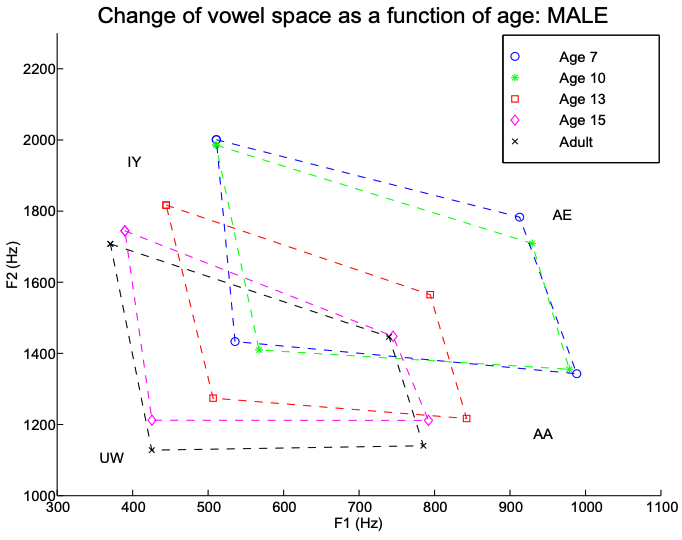
\includegraphics[scale=0.4]{imgs/f1f2children.png}
%\caption{Changes in F1-F2 vowel space as a function of age from \cite{reviewASRchildren}}
%\label{fig:f1f2_children}
%\end{center}
%\end{figure}


\begin{figure}[ht]
\centering
\subfigure[Changes in F1-F2 vowel space as a function of age]{\label{fig:f1f2_children}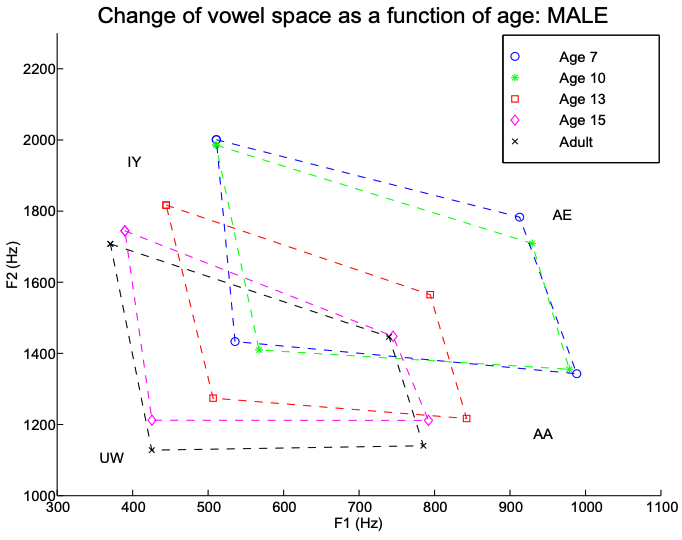
\includegraphics[width=0.48\textwidth]{imgs/f1f2children.png}}
\subfigure[Mean cepstral distance between the two repetitions of the same vowels]{\label{fig:intra_children}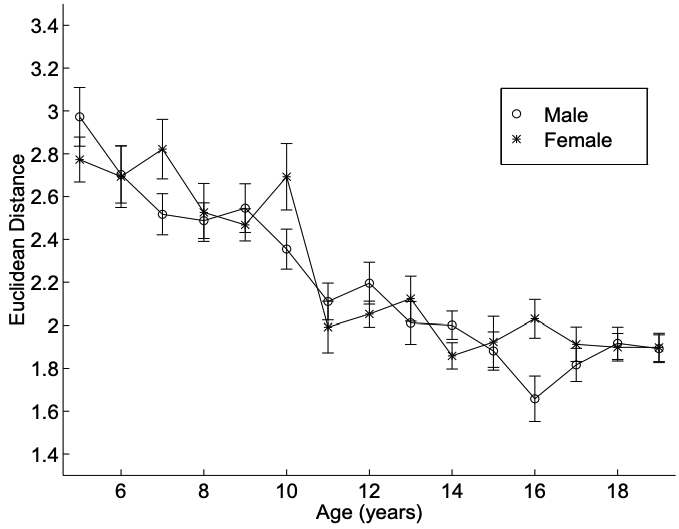
\includegraphics[width=0.48\textwidth]{imgs/intraspeakervariability.png}}
\caption{Formant and cepstral variability. Figures taken from \cite{reviewASRchildren}}
\end{figure}

\begin{figure}[ht]
\centering
\subfigure[Averaged-vowel duration across all vowels and subjects in each age group]{\label{fig:duration_vowel_children}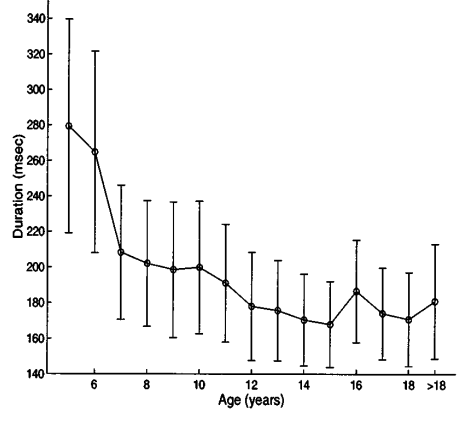
\includegraphics[width=0.48\textwidth]{imgs/children_vowel_duration.png}}
\subfigure[Within- and between-subject variations. The between-subject variation is reduced by a factor of 2.0]{\label{fig:intra_duration_children}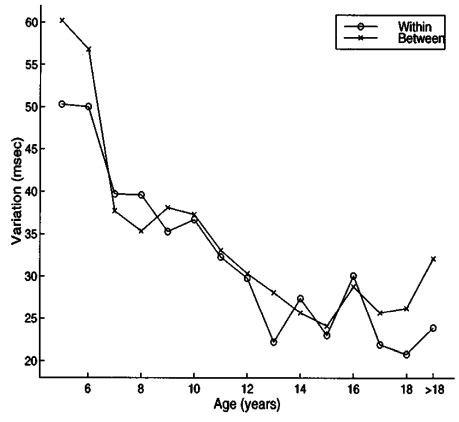
\includegraphics[width=0.48\textwidth]{imgs/Intra_inter_duration.png}}
\caption{Segmental duration variability. Figures taken from \cite{Acoustic_change_children}}
\end{figure}


In addition to inter-speaker variability, \cite{Acoustic_change_children} also highlight the fact that children's speech exhibits intra-speaker variability, signifying that the speech of the same individual can exhibit variations in different ways. This variability arises from two primary sources. Firstly, as previously discussed, the acoustic characteristics of a same children can significantly differ at different ages due to the ongoing growth of their vocal apparatus.  Secondly, even at the same age, the same child may produce variable speech, even when articulating the same vowel. As depicted in Figure \ref{fig:intra_children}, the average cepstral distance between two repetitions of the same vowels by the same child tends to decrease with age, particularly after the age of 10. This reduction in intra-speaker variability is attributed to the progressive mastery of speech articulation components as children grow and refine their motor skills abilities. The decrease in cepstral distance suggests a more coherent and standardised articulation of vowels over time.

%In addition to inter-speaker variability, children's speech exhibits intra-speaker variability, meaning that the same individual's speech can vary in different ways. This variability arises from two sources. Firstly, as previously discussed, the acoustic characteristics of the same child can significantly differ at different ages due to the growth of their vocal apparatus over time. Secondly, even at the same age, the same child may produce variable speech, even when articulating the same vowel. As depicted in Figure \ref{fig:intra_children}, the average cepstral distance between two repetitions of the same vowels by the same child decreases with age, particularly after the age of 10. This reduction is attributed to the progressive mastery of speech articulation components.

% Duration segments for children are longer
Segmental duration is another important aspect of human speech. A segment, as defined by Crystal \cite{segment_definition}, is: \textit{"Any discrete unit that can be identified, either physically or auditorily, in the stream of speech"}. These segmental durations could be vowel or sentence duration. Vowel duration, in particular, is of significant importance in Vowel discrimination. Research, as presented in \cite{Acoustic_change_children}, investigates how these characteristics change in children's speech. As demonstrated in Figure \ref{fig:duration_vowel_children}, the average vowels duration in children exhibits variations with age. On average, younger children tend to have longer vowel durations, resulting in a slower speaking rate. However, as children become more comfortable with the processes of speech production as they age, vowel duration gradually decreases. Similarly to children frequency variations, segmental duration exhibits intra-speaker variability, as illustrated in Figure \ref{fig:intra_duration_children}.

%Segmental duration is another important aspect of human speech. A segment, as defined by Crystal \cite{segment_definition}, is: \textit{"Any discrete unit that can be identified, either physically or auditorily, in the stream of speech"}. These segmental durations could be vowel or sentence duration. The literature emphasizes the significance of vowel duration in vowel discrimination. Research, as presented in \cite{Acoustic_change_children}, investigates how these characteristics change in children's speech. As demonstrated in Figure \ref{fig:duration_vowel_children}, the average duration of vowels in children varies with age. On average, younger children tend to have longer vowel durations, resulting in a slower speaking rate. However, as children become more comfortable with speaking processes with age, vowel duration gradually decreases. Similarly to children frequency variations, segmental duration exhibits intra-speaker variability, as illustrated in Figure \ref{fig:intra_duration_children}.

% Conclusion on frequency challenges 
In conclusion, dealing with both intra- and inter-speaker variability in children's speech, particularly in those under the age of 15, poses a substantial challenge for developing high-performance speech processing models, especially in the context of ASR, where the age of the child is often unknown. In addition, the dynamic processes of vocal tract growth, changes in speech components, and the maturation of speech motor control in children occur simultaneously and overlap, making it considerably more challenging to accurately disentangle and model their acoustic effects. The intricate nature of children's speech, marked by age-related variations in frequency, formants, and segmental duration, underscores the necessity for sophisticated and adaptive models that can accommodate the unique characteristics of these speakers.

%In conclusion, dealing with both intra- and inter-speaker variability in children's speech, particularly in those under the age of 15, poses a substantial challenge for developing high-performance speech processing models for children, especially in the context of ASR, where the age of the child is often unknown. Moreover, the processes involved in speech development in children, including the growth of vocal tract structures, changes in speech components, and the maturation of speech motor control, are simultaneous and overlapping. This development makes it considerably more challenging to disentangle and model their acoustics effects accurately.


\subsection{Language and phonetic knowledge} %************************************************
\label{subsection:mispron}
% Intro on language and phonetic
Language is a complex and multifaceted system of communication that involves the use of symbols, such as words to convey meaning. It is a uniquely human ability and serves as a fundamental aspect of human cognition and social interaction. Linguists have identified five basic components of language \cite{moats2000speech}, including phonology (sounds), morphology (struce and construction of words) , semantics (meaning), syntax (grammar and sentence structure), and pragmatics (how language is used in context). It allows individuals to express thoughts, share information, and engage in social interactions. It is important to note that, languages vary across cultures and regions, exhibiting a rich diversity of sounds, structures, and expressions. Additionally, language can be spoken, written, or signed, and evolves over time. For children, the mastery of language is crucial milestone in their cognitive development, and language plays a central role in shaping culture, identity, and the transmission of knowledge to them. The children's ability to use language effectively develops with age, achieving adult capabilities around the age of 13 , as indicated by research \cite{Acoustic_change_children}. This progression enables the children to transition from producing simple sounds and words to generating more complex sounds and fully articulated sentences.

%Speech is hierarchically composed of sentences, words and phonetic units. Language refers to the cognitive processes of understanding and selecting the appropriate words or phonetic units to convey meaning, as well as arranging these words into coherent sentences. Children's ability to use language effectively develops with age, achieving adult capabilities around the age of 13 \cite{Acoustic_change_children}, enabling them to transition from producing simple sounds and words to generating more complex sounds and fully articulated sentences.
% Explain what are the main disfluency
During the learning process of language acquisition, children, constrained by their limited and developing linguistic knowledge, often make pronunciation errors and encounter disfluencies \cite{language_children}. According to \cite{clark1977psychology}, these errors may include a variety of phenomena, such as:
\begin{itemize}
    \item \textbf{Substitution}:  Involves the inadvertent replacement of the correct pronunciation of an entire word with an alternative rendition.
    \item \textbf{Omission}:  Refers to the act of leaving out or neglecting a part of speech, a word, or a phrase that would typically be included in a grammatically correct or complete sentence.
    \item \textbf{Mispronunciation}:  Involves the act of pronouncing a word or a part of a word incorrectly, deviating from the standard or expected pronunciation in a particular language or dialect.
    \item \textbf{Pause and Hesitation}: Entails temporary breaks or delays in speech during which a speaker might refrain from producing sound or articulate speech in a hesitant manner.
    \item \textbf{Filler and mumbling}:  Filler encompasses linguistic elements used during pauses or hesitations when a speaker needs time to think, including unintelligible sounds, words, or phrases without significant meaning. Mumbling is characterised by unclear or indistinct speech, often marked by low volume, unclear articulation, and imprecise pronunciation.
    \item \textbf{False-start}:  Refers to an instance where a speaker begins a sentence or an utterance and then stops abruptly before completing it. This interruption is often followed by a restart or a correction to articulate the intended message more accurately.
    \item \textbf{Sound-out}: Involves a pronunciation strategy in which a speaker articulates a word by pronouncing each sound or phoneme separately, rather than blending them together seamlessly.
\end{itemize}

%\begin{itemize}
%    \item Substitution: Incorrectly pronouncing an entire word 
%    \item Omission: Not pronouncing an entire word
%    \item Mispronunciation: Incorrectly pronouncing some part of a word
%    \item Pause and Hesitation: Partially pronouncing a word
%    \item Filler and mumbling: Using unintelligible speech or noise as filler for hesitation or pause 
%    \item False-start: Stop and start a sentence in the middle of one
%    \item Sound-out: Pronouncing word as a sequence of distinct units rather than continuous sounds
%\end{itemize}
% Give more example of disfluency over age
Potamianos and Narayanan's study \cite{language_children2} revealed significant insights into the variability and characteristics of children's linguistics. They found that inter-speaker variability is approximately twice as much as intra-speaker variability. Additionally, their research found that the rate of mispronunciations is twice as high for children aged 8 to 10 compared to those aged 11 to 14. Conversely, the trend is reversed for filler pauses, where the older group exhibits a higher rate. Furthermore, younger children, of 8 to 10 years, tend to produce more false starts and breathing.
%Potamianos and Narayanan \cite{language_children2} found that inter-speaker variability is about twice more than intra-speaker variability. They also showed that there is twice more mispronunciation for children of 8 to 10 years old compared to children of 11 to 14, while the trend was reversed for filler pause. Furthermore, younger children also produce more false starts and breathing.

% Explain that it is hard to model, that adaptation from adult because Children has different grammatical constructs 

Mispronunciations and disfluencies are not necessarily present in adult speech to the same extent as in children's speech, as supported by studies such as \cite{Children_language_model,children_language_model2}. These studies used language models specifically trained on children's speech, demonstrating the advantages over the use of adult language models. The findings underscored the differences between children's and adults's linguistics, encompassing variations in grammatical structures as well as the presence of mispronunciations and disfluencies. Such insights are crucial for the development of effective language models tailored to the unique characteristics of children.
%Mispronunciation and disfluencies in children's speech are not necessarily present in adult speech. This statement was proven by \cite{Children_language_model,children_language_model2}  employing a language model trained on children's speech and demonstrating the benefits over the use of adult language models. Demonstrating that children's language differs from adults in terms of grammatical structures, mispronunciation, and disfluencies.


\subsection{Data scarcity}%****************************************************************
\label{section:data_scarcity}
% Data is key in this deep learning time
In recent years, the emergence of deep learning has brought about significant advancements in the ASR field. The combination of increased computational power and the abundance of available data has played a pivotal role in driving these improvements. The success deep learning is largely attributed to the deep neural networks (DNNs), which effectively approximate the complex non-linear functions. With the help of the capability, DNNs excel in capturing intricate patterns and representations in speech data, contributing to more accurate and robust ASR systems. However, the efficacy of a DNN in capturing intricate speech patterns depends a lot on the availability of a substantial amount of training data. The emphasis on accumulating expansive datasets is driven by the recognition that a large of diverse and comprehensive training data is pivotal for enhancing the capabilities and generalization of DNN-based ASR systems. Notably, top-performing ASR systems like Whisper have been trained on extensive datasets, surpassing 680,000 hours of data collected from the web \cite{radford2023robust}. There is a noticeable trend in the speech research community towards the collection of larger datasets, exemplified by initiatives such as the LibriSpeech dataset, which comprises around 1,000 hours of speech \cite{librispeech}, and the GigaSpeech dataset, featuring a staggering 10,000 hours \cite{chen2021gigaspeech}.

% Explain pb with children dataset
Unfortunatly, despite rare recent efforts to collect larger children datasets \cite{MyST,singakids,ahmed2021auskidtalk}, the majority of publicly available children corpora include fewer than fifty hours of speech. This is significantly less than a typical adult speech corpora, which usually contains hundreds or even thousands of hours of data. Furthermore, the majority of the accessible children's data are English corpus \cite{MyST,cmu,cslu,pf-star-british,ahmed2021auskidtalk}. However, English is a large-size, resource-rich pluricentric language which should be seen more as an exceptional case, rather than an average representative. A compilation of existing datasets containing children's speech will be presented in \ref{section:children_corpora}.

% Ethical problems
The scarcity of children's speech datasets availability can be attributed to a combination of ethical, legal, and technical challenges. Collecting speech data from children raises ethical concerns related to obtaining informed consent, ensuring privacy, and protecting minors. The heightened awareness of online safety and security concerns further complicates the creation and sharing of datasets that include children's speech, as there is a need to safeguard against potential misuse and ensure the anonymity of participants.
% Need of a diversity
Beyond ethical and legal considerations, technical challenges also play a role. Children's speech patterns, language development, and pronunciation can vary significantly across different age groups, as explained in previously, making it challenging to create datasets that accurately represent the diversity of children's speech. Moreover, the resource-intensiveness of collecting high-quality speech data from children, which involves careful planning, recruitment efforts, and coordination with schools or parents, can further contribute to the limited availability of such datasets.
% age problem, school recording -> noise, attention span of the children
Finally, collecting speech data from children is a challenging and time-consuming task. Various factors can significantly impact the quality of the gathered speech. These include children's short attention spans, recording environments that might be noisy (such as a classroom), and the quality of the speech, which is highly dependent on the task at hand (reading tasks are generally more complex for children).

% explain that with data, a lot of problems can be solved
The importance of having a large database of children's speech to encompass greater variability has been emphasised in a study conducted by Liao in 2015 \cite{asr-google}. In this work, the researchers addressed the limited availability of extensive children's speech datasets by training an ASR model using a sizable in-house corpus of children's speech. Notably, this corpus was comparable in size to typical adult speech corpora. The result was the attainment of state-of-the-art performance by the ASR model, demonstrating competitiveness with adult speech recognition systems. This study underscores the crucial role of comprehensive and diverse children's speech datasets in developing robust and high-performance ASR models tailored to the distinctive characteristics of children's speech.
%The need for a large database of children's speech to cover a higher variability has been proven by \cite{asr-google}.  In this work, the authors trained an automatic speech recognition model using a large in-house corpus of children's speech, comparable in size to an adult speech corpus. This resulted in state-of-the-art performance competitive with adult speech recognition systems.



\newpage
\section{Introduction to automatic speech recognition}%----------------------------------------------------------- ~11 pages
In this section, a brief historical overview of ASR is presented, laying the foundation for a subsequent exploration of predominant trends and modules within ASR systems. This comprehension is necessary for the following sections of this thesis. While not exhaustive, this overview provides essential insights, with certain topics falling beyond the scope of this thesis are intentionally omitted. For a more exhaustive understanding of ASR, readers are encouraged to consult references such as \cite{benzeghiba2007automatic, karpagavalli2016review, arora2012automatic}. The section is structured as follows: Firstly, we present the historical evolution of ASR, followed by an description of traditional ASR systems, succeeded by an explanation of the end-to-end paradigm. Concluding this section, a discussion on automatic speech recognition metrics is presented.

%In this section, we provide an overview of the main trends and modules of automatic speech recognition systems, as this understanding is necessary for the rest of this proposal. This overview is by no means exhaustive, and some subjects that are outside the scope of this thesis are excluded. More thorough information regarding ASR can be found in \cite{benzeghiba2007automatic,karpagavalli2016review,arora2012automatic}. This section is divided as follows: First, we will present traditional ASR systems, and then we will explain the end-to-end paradigm for ASR. Finally, we will present automatic speech recognition metrics.
\subsection{A brief history of Automatic Speech Recognition}

\subsubsection{Early Days}

The origins of speech recognition technology can be traced back to the 1950s and 1960s, with initial projects focusing on isolated word recognition in a speaker-dependent context. One of the earliest project in this domain was the creation of a digit recognizer at Bell Telephone Laboratories in 1952. This recogniser demonstrated the automatic recognition of telephone-quality digits spoken at normal speech rates by a single adult male, achieving an impressive accuracy of up to 99\%. The system relied on formant frequency approximations to recognise entire words. It is impotant to underscore that within this recogniser, there was an absence of explicit modeling of syllables, consonants, vowels, or any other sub-word units. In this recogniser, a word was treated as a single unit, which was then compared with ten standard digit patterns to find the best match. The recognition process first involved extracting two frequency ranges, below and above 900 Hz. Motivated by the observation that these two frequency ranges approximately align with the frequencies of the first two formants in speech. Then, these formant approximations were plotted on a 2D-plot with a trace interruption period of 10ms. Finally, when presented with new audio, the system generated a plot, compared it to the reference plots of the ten digits, and returned the closest match by computing the highest relative correlation coefficient. Figure \ref{Bell} illustrates an example of the 2D representation of the ten digits.

%The first projects for a technology that resembles to speech recognition date back to the 1950s-1960s. At this time, the work focused on isolated word in a speaker dependent context. The earliest project was a digit recognizer created at Bell Telephone Laboratories in 1952. This recognizer automatically recognize telephone-quality digits spoken at normal speech rates by a single adult-male individual, and obtained an accuracy up to 99\%. This system relied on formant frequency approximations to recognise whole word. No model of syllables, consonants, vowels or any other sub-word units are present in this recognizer. The word was treated as a single unit, and compared with ten standard digit patterns to find the best match. In order to do this the circuit extracted two frequency ranges, frequencies below and above 900 Hz. These two frequency ranges roughly approximate with the first two formants of speech. Then, these two formants approximation are plotted on a 2D-plot with a trace interruption period of 10ms. Finally, when a new audio is provided to the recognizer the newly generated plot is compared the to ten references plots of the ten digits and the closest match is return by computing the highest relative correlation coefficient. Figure \ref{Bell}  shown an example of the 2D representation of the ten digit.

\begin{figure}[h]
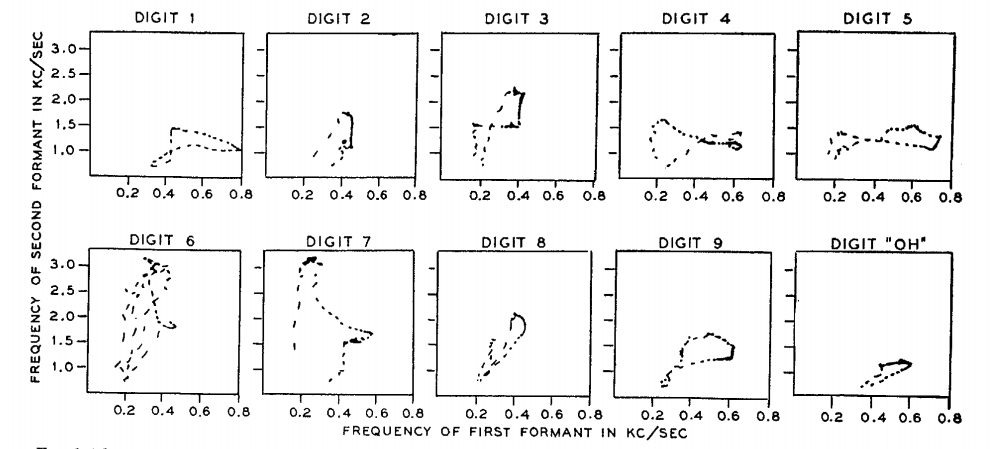
\includegraphics[width=\textwidth]{imgs/bell.png}
\caption{Example of a standard digit pattern from Davis et al. 1952}
\label{Bell}
\end{figure}
%Later,in 1962, IBM developed Shoebox, a device that recognize 16 spoken words, the ten digits and command words such as "plus", "minus" and "total" using a similar pattern matching algorithm.


In 1962, IBM developed Shoebox, a device capable of recognising 16 spoken words, including the ten digits and command words such as "plus," "minus," and "total." This system employed a pattern-matching algorithm similar to the pattern-matching approach used in the Bell Telephone Laboratories's recogniser.

%Nonetheless, extended such a system for large vocabulary recognition would be not possible. This template-matching approach required each word representation to be saved on disk and compare the unknown spoken word with all this representations. When extend this approach to a larger vocabulary, the time and disk usage complexity become an issue. In addition, in order for the circuit to deliver an accuracy of the same range for a new speaker, a preliminary analysis of the speech of this individual and circuit adjustment is required.

Nevertheless, extending such a system for a larger vocabulary would be impractical. Indeed, the template-matching approach necessitated saving each word representation on disk and comparing the unknown spoken word with all these representations. Therefore, when attempting to scale this approach to automatic large vocabulary recognition, issues of time and disk usage complexity emerged as significant challenges. Furthermore, in order for the circuit to deliver an accuracy of the same range for a new speaker, a preliminary analysis of the speech of that individual and subsequent circuit adjustments were necessary. These limitations underscored the need for more scalable and adaptive approaches and led the field of automatic speech recognition to continued to evolve.

 

\subsubsection{The Speech Understanding Research program}

%In the early 1970s, after the initial success of pattern matching algorithms for single word recognition, the Advanced Research Program Agency of the U.S. department of Defense, ARPA, funded a five-year program Speech Understanding Research (SUR). The goal was to "obtain a breakthrough in speech understanding capability that could then be used toward the development of practical man-machine communication system ". It is in the context of this program that four different research groups have been funded: two groups from Carnegie-Mellon University (CMU), one from Bolt Beranek and Newman Inc. (BBN Hwim) and the last one from System Development Corporation (SDC). For each group, they were given a different task: Facts about ships, travel budget management and document retrieval. Where the  end goal task was to create a system that can recognize simple sentences in the context of the task from a vocabulary of 1,000 words with a 10\% WER in a reasonable time. 

In the early 1970s, subsequent to the initial success of pattern matching algorithms in single-word recognition, the Advanced Research Program Agency of the U.S. Department of Defense, ARPA, initiated funding for a five-year program called Speech Understanding Research (SUR). The overarching goal of SUR was to "obtain a breakthrough in speech understanding capability that could then be used toward the development of practical man-machine communication system ". Within the context of this program, four distinct research groups were funded: two from Carnegie-Mellon University (CMU), one from Bolt Beranek and Newman Inc. (BBN Hwim), and the last one from System Development Corporation (SDC). Each group was assigned a specific task, such as dealing with facts about ships, travel budget management, and document retrieval. The ultimate objective for each group was to create a system capable of recognising simple sentences within the context of their assigned task, from a vocabulary of 1,000 words, achieving a Word Error Rate (WER) of 10\% in a reasonable amount of time.


%They realised that the pattern matching word identification strategy could not be applied to the problem of sentence understanding and they had to redesign the single word identification system. First of all, acoustic characteristics of words can vary considerably depending on the context of the sentence; the phonetic and phonological processes of English. Storing on disk each  words and all his different variations was not possible. In addition, discovering each words boundaries was almost impossible and compute the pattern-matching, even if the word boundaries were found, would be long and would not fit in the reasonable time requirement. Indeed, the system would compare the query word with each of the 1,000 words stored and all the possible variations. Secondly, output sentence length is variable and unknown, which is not the case in a single word identification. Therefore it was decided to use a smaller unit than the word to model speech, the phonemes. The phonemes are the smallest distinctive and meaningful unit that compose speech. For each language is associated a set of finite number of phoneme, usually under 50, that can be use to create words.


The realisation that the pattern-matching word identification strategy could not be directly applied to the challenge of sentence understanding prompted a redesign of the single-word identification system. In the first hand, one key recognition was that the acoustic characteristics of words can vary considerably based on the context of the sentence. The impracticality of storing each word and all its possible different variations on disk became apparent. Moreover, determining the boundaries of each word  was an almost impossible task, and even if these boundaries were identified, the pattern-matching computation, involving comparisons with each of the 1,000 stored words and all their possible variations, would be time-consuming and exceed the reasonable time requirement. Secondly, another crucial consideration in the redesign of the system was that the length of the spoken sentence is variable and unknown, in contrast to the relatively fixed length in single-word identification tasks. In sentence understanding, the system needed to handle variable sentence lengths, making it necessary to adopt a more flexible approach in modeling and recognizing speech.

To address these challenges, a shift was made to a smaller unit than the word for modeling speech -namely, phonemes. Phonemes are the smallest distinctive and meaningful units that compose speech. Each language is associated with a finite set of phonemes, typically fewer than 50, which can be combined to form words. This shift enabled a more efficient and flexible representation of speech, accommodating the variability in the pronunciation of words.


%Among all proposed systems of the project, the Harpy system, implemented by Lowerre in 1976 for the Carnegie Mellon team, showed the best performances. Harpy is a speaker-specific  system, using pattern matching algorithm at the phoneme level instead of word level. The Harpy system  use a set of 98 phonemes and diphones, a pronunciations of all words and a graph where all accepted sentences are compiled using 15k states.  When a new utterance arrived in the system, it is first low pass filtered at 5kHz, digitized at 10k samples per second, then a 14 linear prediction coefficients are computed with a 10ms shift and group it together similar adjacent acoustic segments to speed-up the decoding process. These audio segments are then compared against the 98 phonemes templates and the best path over the graph is returned. Figure \ref{harpy} show a decoding graph example.
Among all the systems proposed in the project, the Harpy system implemented by Lowerre in 1976 by the Carnegie Mellon team exhibited the best performances \cite{klatt1977review}. Harpy is a speaker-specific system that use a pattern-matching algorithm at the phoneme level instead of the word level. The system employs a set of 98 phonemes and diphones -a pair of consecutive phonemes- , encompassing pronunciations of all words, along with a graph compiling all accepted sentences using 15,000 states. When a new spoken utterance is provided to the system, it undergoes an initial processing phase, involving low-pass filtering at 5 kHz, digitization at 10,000 samples per second, and computation of 14 linear prediction coefficients with a 10ms shift. To speed-up the decoding process, analogous adjacent acoustic segments are grouped together. Subsequently, these audio segments are compared against the 98 phoneme templates, and the system deduces the optimal path over the decoding graph. Figure \ref{harpy} provides an exemplar illustration of a decoding graph in the Harpy system.



\begin{figure}[h]
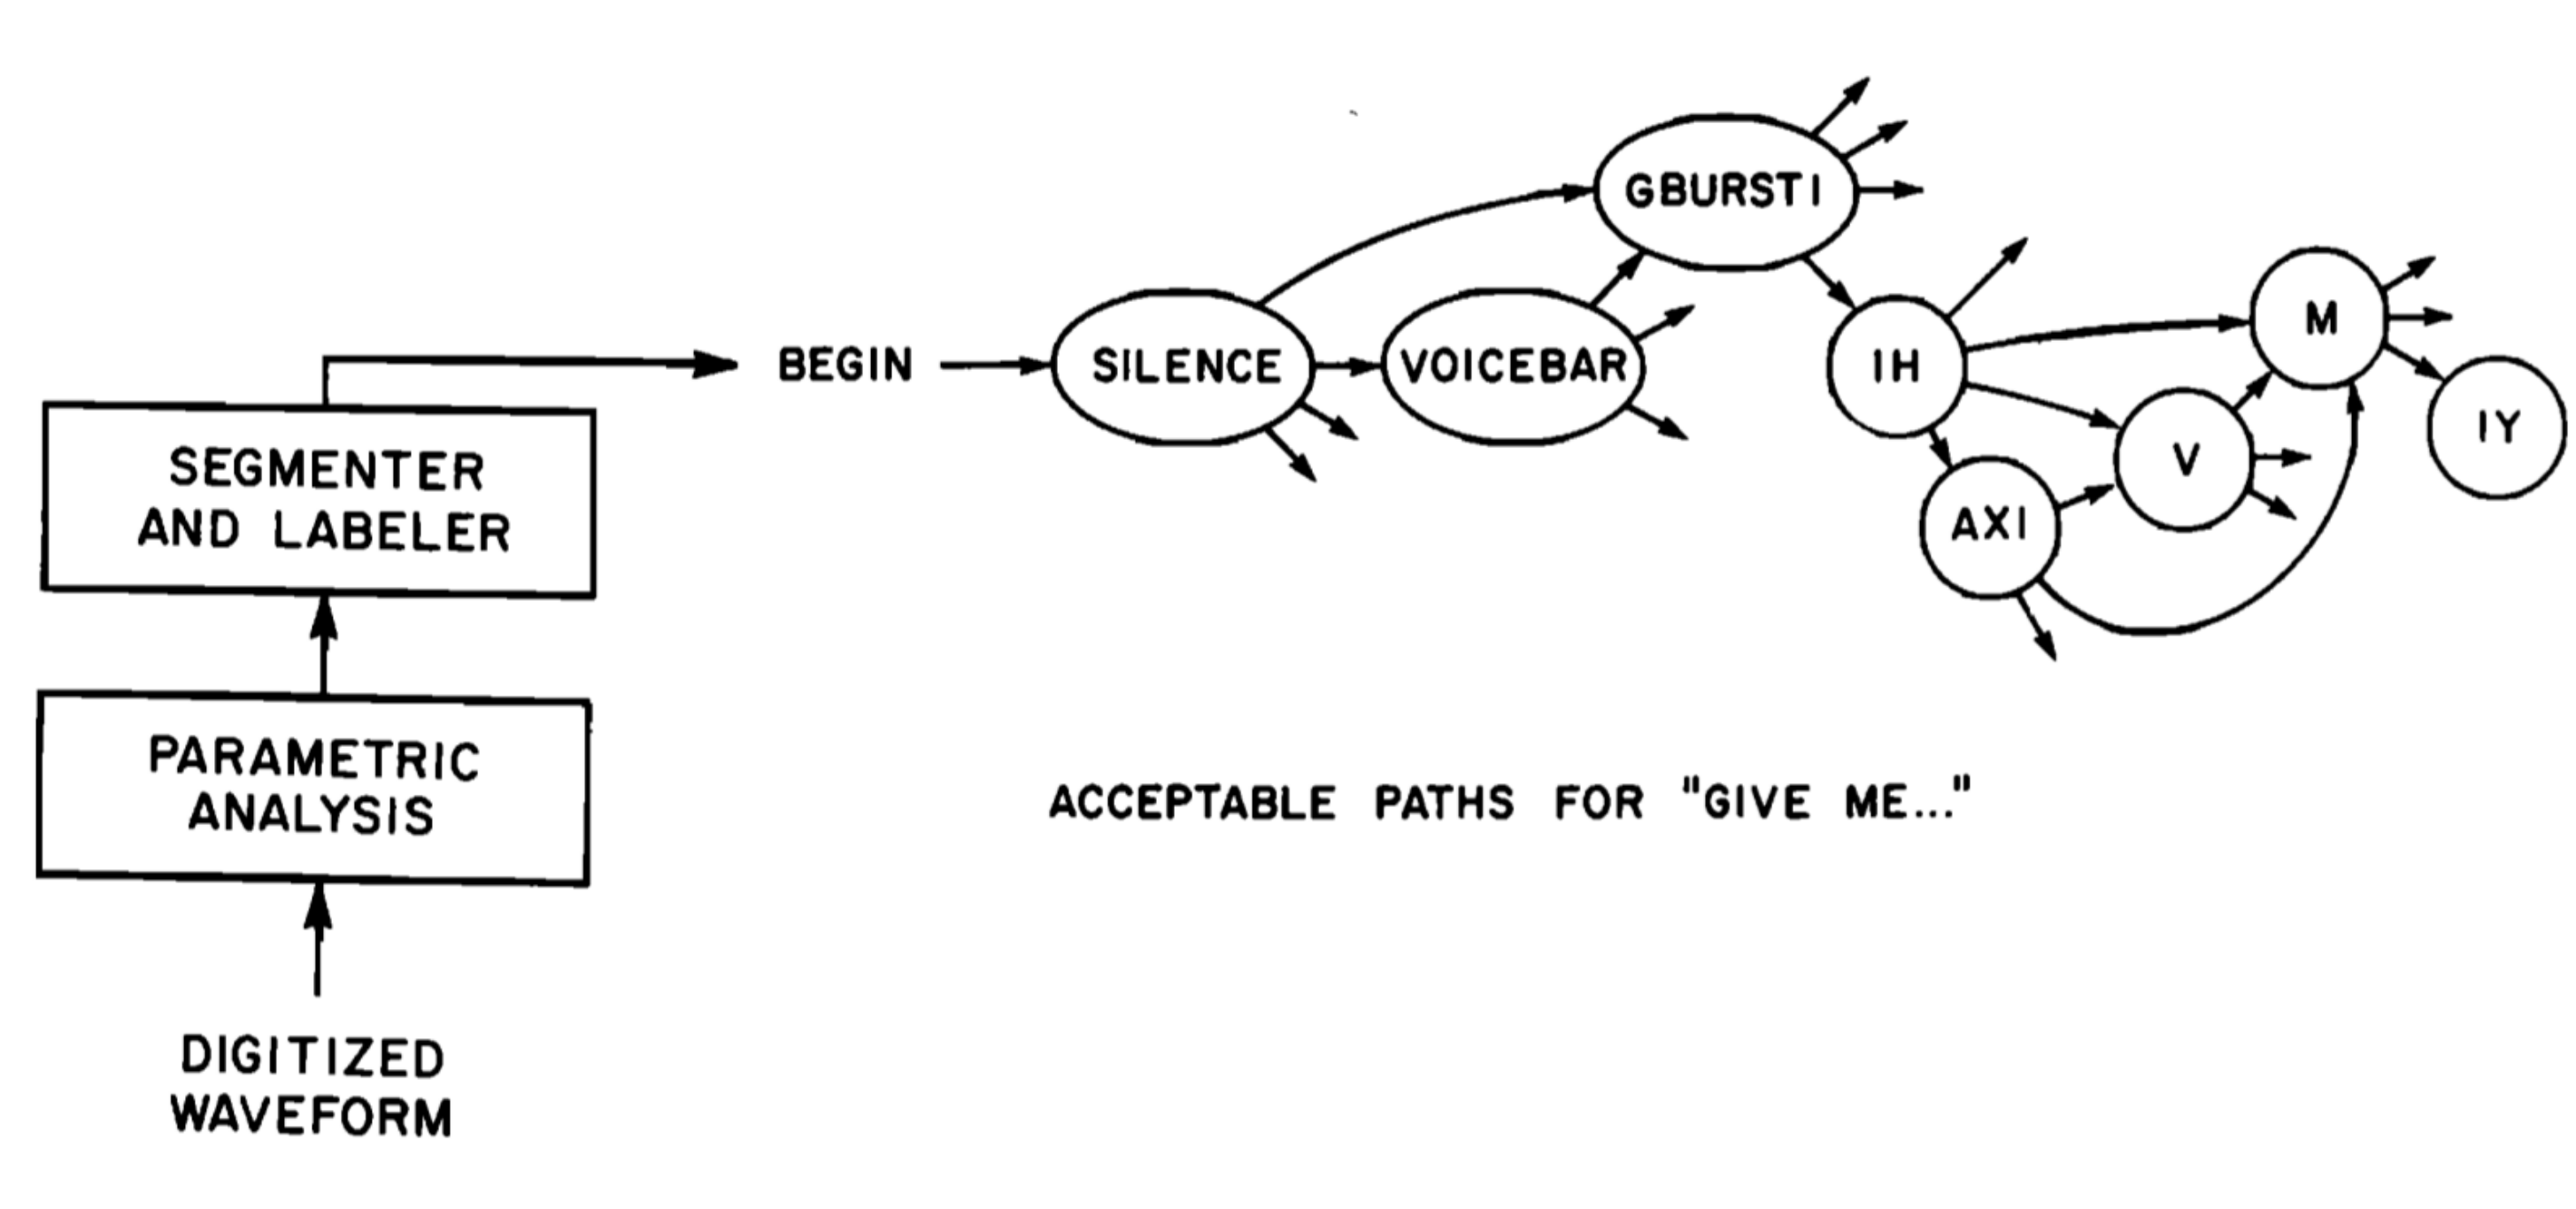
\includegraphics[width=\textwidth]{imgs/harpy.png}
\caption{Example of a decoding graph from the Harpy system for the sentence "GIVE ME" from \cite{klatt1977review}}
\label{harpy}
\end{figure}

%Despite the success of the Harpy system, it is a  speaker-specific system. For a new speaker, the system must be tuned over the 98 phonemes templates. In addition, this system can not understand more the 1,000 words and only use a simple handcrafted grammar, making this system not reliable for spontaneous speech. Finally, the decoding time was far from real time.
Notwithstanding the achievements and success of the Harpy system, it has limitations that hinder its broader applicability. As a speaker-specific system, it requires tuning for each new speaker over the 98 phoneme templates. Additionally, the system is constrained to recognising a vocabulary of no more than 1,000 words and relies on a simple handcrafted grammar, making it less reliable for handling spontaneous speech. Moreover, the decoding time of the system falls short of real-time requirements. These constraints highlight the need for more generalisable and efficient speech recognition systems, especially for handling diverse speakers and spontaneous speech scenarios. Therefore, as research progressed, the limitations of template-based approaches became apparent. This realisation prompted the exploration of probabilistic modeling techniques, marking a shift towards more sophisticated and adaptable approaches in automatic speech recognition. 


\subsection{Traditional automatic speech recognition systems} % ~4 pages %************************
% HMM-DNN
\begin{figure}
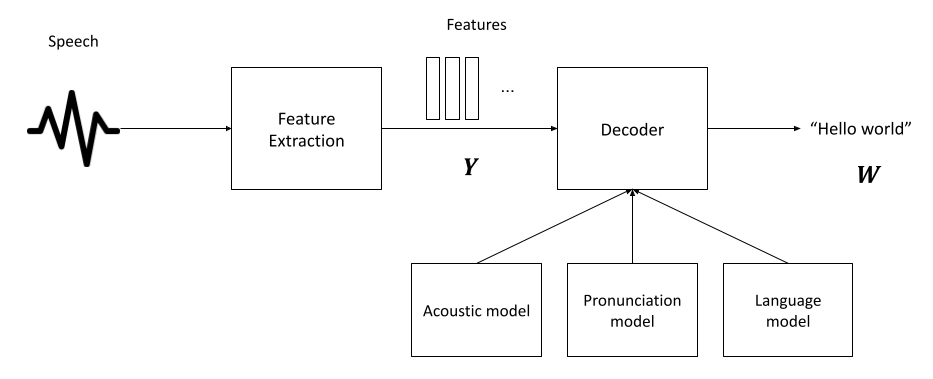
\includegraphics[width=\textwidth]{imgs/HMM-GMM_architecture.png}
\caption{Architecture of a HMM-based speech recognition system}
\label{HMM-GMM-model}
\end{figure}
%The introduction of Hidden Markov Models (HMMs) in the 1970s, Gaussian Mixture Models (GMMs) in the 1980s, and statistical grammars in the 1990s, pushed automated speech recognition research away from pattern matching toward statistical modelling \cite{first_asr}. For example, the Hidden Markov Model Toolkit (HTK) \cite{htk_book}, a toolkit extensively adopted by the community, proposed the first benchmark on DARPA's Resource Management challenge in 1992  \cite{darpa1992}. Those components of the traditional ASR, illustrated in figure \ref{HMM-GMM-model}, are still at the core of modern HMM-based speech recognition systems. Later, ASR systems performances improved significantly as a result of the transition from HMM-GMM to the deep neural networks paradigm HMM-DNN  \cite{hmm-dnn}, called hybrid models.

%What are HMM
In the 1970s, the introduction of Hidden Markov Models (HMMs) led to a paradigm shift in ASR research, moving away from traditional pattern-matching methods towards statistical modelling \cite{first_asr}. Indeed, HMMs are particularly effective at capturing the sequential and temporal nature of speech. They assume that speech can be represented as a sequence of hidden states, each state corresponding to a distinct phonetic unit. HMMs model the transitions between these states and, at each state, generate observable acoustic features. The hidden aspect refers to the fact that the underlying states are not directly observed but inferred from the observable features. HMMs are particularly well suited to modelling speech dynamics, as they can represent the variability of speech sounds over time. In the context of ASR, HMMs have been widely used to model phonemes, words or sub-word units.

%What are GMM
Building on this foundation, the 1980s saw the emergence of Gaussian Mixture Models (GMMs), which further enhanced the statistical modeling capabilities of ASR \cite{htk_book}. GMMs allowed for a more flexible representation of the probability distributions underlying speech features.
GMMs are used to model the statistical distribution of acoustic features associated with each hidden state in an HMM. They assume that the distribution of features can be approximated by a mixture of several Gaussian distributions. GMMs are versatile in capturing the variability of speech sounds, allowing a more flexible representation of the acoustic units. In ASR, GMMs are commonly used to model the emission probabilities associated with each state in an HMM. This means that given a particular state, the GMM provides the likelihood of observing a specific set of acoustic features. By combining the temporal modeling capabilities of HMMs with the statistical representation power of GMMs, this framework effectively captures the complex relationship between acoustic features and phonetic units.

% What are statistical grammars
Finally, in the 1990s, statistical grammars also played a crucial role, providing a structured framework for incorporating linguistic into ASR systems \cite{darpa1992}. Statistical grammars represent a category of grammars that integrate statistical information to characterise the probability of diverse linguistic structures. In contrast to traditional rule-based grammars, which articulate a language's syntax through explicit rules, statistical grammars adopt a data-driven methodology. They assign probabilities to various linguistic constructions based on observed frequencies within a designated corpus.

%What are DNN
The components illustrated in Figure \ref{HMM-GMM-model} represent the traditional ASR pipeline. These components continue to form the core of modern HMM-based ASR systems. However, in more recent times, the field of ASR has witnessed a transformative shift with the adoption of deep neural networks (DNNs) instead of GMM. Called hybrid models, they combining the strengths of HMMs and DNNs and  have further improved the ASR system performance \cite{hmm-dnn}. A DNN is a subtype of artificial neural networks consisting of multiple layers of interconnected neurons. These neurons, organised in layers, receive an input signals, and each connection between neurons is characterised by a weight that signifies its strength. In addition, each neuron is associated with a bias, provide an additional learnable parameter. During training, the network adjusts these weights and biases to minimise the difference between predicted and actual outputs, a process known as backpropagation. Moreover, there is a non-linear activation functions within neurons, as it enables the network to model intricate, non-linear patterns of the data. The weights, biases and non-linearity allow DNNs to capture complex relationships and representations from the data,learning hierarchical features and abstracting information across multiple layers of the network.

%Math formulation
In this statistical framework, the continuous speech audio waveform is transformed into a sequence of fixed-size acoustic vectors, denoted as $\boldsymbol{X}=x_1,...,x_T$. The goal of the Automatic Speech Recognition (ASR) system is to determine the sequence of words, $\boldsymbol{w}=w_1,...,w_L$ ​, that is most likely to have produced the observed acoustic vector sequence $\boldsymbol{X}$. This is formulated as finding the word sequence $\hat{w}$ that maximises the conditional probability $P(\boldsymbol{w}|X)$. More formally:
%In this statistical framework, the continuous speech audio waveform is converted to a sequence of fixed size acoustic vectors $\boldsymbol{X}=x_1,...,x_T$. Then the ASR system tries to find the sequence of words $\boldsymbol{w}=w_1,...,w_L$ which is most likely to have generated $\boldsymbol{X}$. More formally:
\begin{equation} \label{equation:asr_0}
    \boldsymbol{\hat{w}} = \argmax_{\boldsymbol{w}} \{P(\boldsymbol{w}|X)\}
\end{equation}
However, directly modeling the conditional probability $P(\boldsymbol{w}|X)$ can be challenging. Bayes' Rule offers a way to express this probability in terms of more manageable components, specifically by decomposing it into the product of the likelihood of the observed acoustic vector sequence given the word sequence $P(X|\boldsymbol{w})$ and the prior probability of the word sequence $P(\boldsymbol{w})$. Therefore, equation \ref{equation:asr_0} became:
%However, this probability is difficult to model directly, but using Bayes' Rules gives:
\begin{equation}  \label{equation:asr}
    \hat{\boldsymbol{w}} = \argmax_{\boldsymbol{w}} \{\frac{P(X|\boldsymbol{w})P(\boldsymbol{w})}{P(X)}\} =\argmax_{\boldsymbol{w}} \{P(X|\boldsymbol{w})P(\boldsymbol{w})\}
\end{equation}
Here,  the likelihood $P(\boldsymbol{X}|\boldsymbol{w})$ is determined by the acoustic model component, capturing the probability of observing the acoustic vector sequence $\boldsymbol{X}$ given the word sequence $\boldsymbol{w}$. In parallel,  the prior probability $P(\boldsymbol{w})$ is determined by the language model component. The term $P(X)$ is not essential for determining the maximum probability and can be omitted in the context of finding the most likely word sequence. Subsequent sections will provide a more in-depth exploration of these distinct components and their processes.
%Here, the likelihood $P(\boldsymbol{X}|\boldsymbol{w})$ is determined by the acoustic model component while $P(\boldsymbol{w})$ is determined by the language model component.  As $P(X)$ is not required to determine the maximum, it can be omitted. The following sections describe the different components and processes in more detail.

% Feature extraction 
\subsubsection{Feature extraction}%*********************************************************
%The feature extraction component's purpose is to extract useful information about the speech's linguistic content. To this end, at each time step, the continuous waveform is transformed into a small fixed-size vector. An acceptable approximation is that speech is considered stationary on the period covered by a single vector. As a result, feature vectors are generally generated every 10-milliseconds with a 25-millisecond overlapping window.
The feature extraction component plays a crucial role in capturing pertinent information about the linguistic content of speech. Its primary objective is to transform the continuous waveform of speech into a compact sequence of fixed-size vectors. A common assumption is that speech can be treated as stationary within the time span covered by a single vector. Consequently, feature vectors are typically computed at intervals of 10 milliseconds, often with a 25-millisecond overlapping window.

\begin{figure}
    \begin{center}
    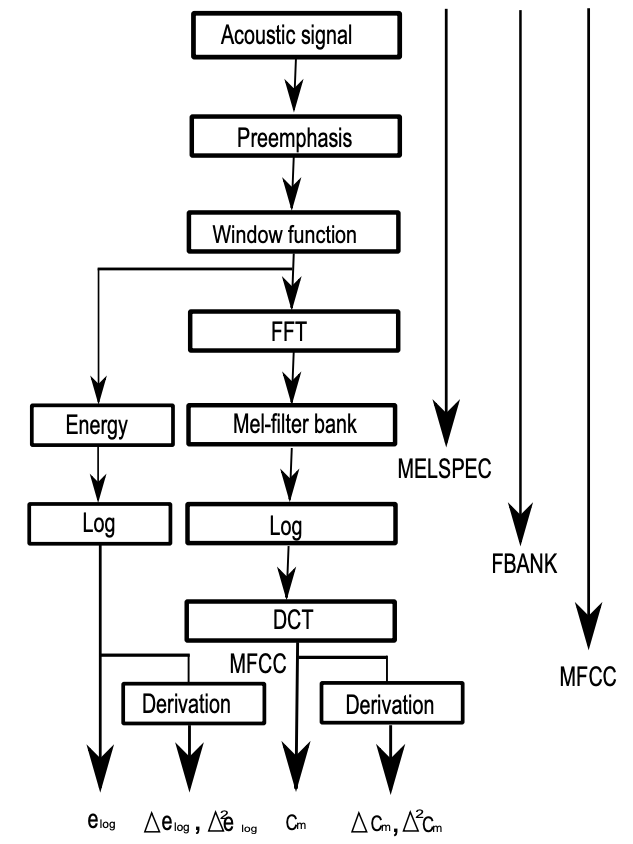
\includegraphics[scale=0.3]{imgs/features.png}
    \caption{Principal block scheme of main speech features for ASR: Melspec, fbanks and MFCC coefficients from \cite{kiktova2013comparison}}
    \label{feature_block}    
    \end{center}
\end{figure}

% MFCC
Mel-frequency cepstral coefficients (MFCCs) \cite{mfcc} are the most widely used features for speech recognition on HMM-GMM and HMM-DNN systems. These are generated by: i) Computing the spectrum of the windowed speech signal by using a discrete-time Fourier transform. ii) Then convoluted with triangular Mel filters (usually 20, called filterbanks), where those filters are narrow in the lower frequencies and wider in higher frequencies, which is similar to the human cochlea. iii) A log transformation is applied. iv) In order to decorrelate the filterbank energies a discrete cosine transform (DCT) is used. Note that some HMM-DNN models are using the filterbanks from ii) directly as input features.
% 

%Delta features and concatenation
For each time step, the feature vector only contains information about the current speech window. It does not, however, provide information on the dynamics of the signal. To bring to these spectral coefficients some context, the first and second-order derivatives are concatenated ($Delta$ and $Delta$, respectively). These first-order derivative coefficients are calculated as follows:
\begin{equation}
 \label{equation:delta}
    \Delta_i = \frac{\sum^{N}_{n=1}n(f_{i+n} - f_{i-n})}{2 \sum^N_{n=1}n^2} \\
\end{equation}
Where the $f_i$ is the feature at the instant $i$. Usually, $n$ is equal to 2. Furthermore, the second-order derivate $\Delta\Delta$, also written $\Delta^2$, can be computed using the same calculation \ref{equation:delta} by replacing the spectral feature $f_i$ by the first-order derivative $\Delta_i$. Thus, the concatenation of the derivatives $\Delta$ and $\Delta^2$ features with the spectral features is denoted $\boldsymbol{x_i}$ as follows:
\begin{align}
    \boldsymbol{x_i} = [x_i^T \qquad \Delta_i^T \qquad \Delta^{2^T}_i]^T
\end{align}
% What is an Acoustic model
\subsubsection{Acoustic model}%****************************************************************
% There role and limitation of simple AM
The role of the acoustic model (AM) is to determine $P(\boldsymbol{X}|\boldsymbol{w})$. In other words, identify which phone or none was uttered in each frame. The most straightforward method would be to use any classifier, such as GMM models with one GMM per phone. However, such a classifier does not account for the temporal dependencies of speech (co-articulation). Indeed, to properly categorize each frame, the current frame and its context (previous and following frames) are necessary. In addition to co-articulation, there is an acoustic difference at the beginning, middle and end of each phone.
Therefore, the HMM framework has been presented as a solution to these concerns \cite{Dragon_system}. Indeed, HMM provide temporal flexibility (e.g., self-looping) as well as a well-understood framework with effective learning (Expectation Maximization) and decoding (Viterbi) algorithms. 

% Use of HMM and HMM-GMM
In the HMM terminology, the observed variables are called observations (here, the acoustic features), while the hidden variables are referred to as states. The states are generated using a first-order Markov process, where the $i^{th}$ state $S_i$ is only dependent on the previous state $S_{i-1}$. It is assumed that all observations are independent given the states that generated them. To better model acoustical differences, one phoneme is typically represented by a three states linear HMM (generally the beginning, middle and end of the phoneme). Finally, with HMM-GMM, each state is modelled by a GMM to determine the likelihood of the observation in that state (i.e. determine if the speech segment matches the phoneme pronounced). A monophone GMM-HMM contains one model for one phoneme. For example, since English has 44 phonemes \cite{bizzocchi2017many}, a monophone system on English will have 44 separate GMM-HMMs. However, monophone systems are limited to modelling natural speech in its full complexity. This is due to co-articulation effects, in which the pronunciation of a phoneme is influenced by its context. Therefore, ideally, there would be a model for every phoneme in every phonetic context. In other words, the phoneme with its left and right context. Such system is called a triphone system. Consequently, there should be $N^3$ models to train for a language with $N$ phonemes. For instance, as English has 44 phonemes, there should be $44 * 44 * 44$ or 85,184 models. Since there is not enough data to see all these contexts, they are clustered using a decision tree.

% HMM-DNN
The idea of hybrid models emerged in the 1990's with the usage of multi-layer perceptrons (MLP) as substitutes for GMMs in HMM-GMM system \cite{bourlard2012connectionist,meinedo2003audimus}. In 2012, the use of deep neural networks (DNN), MLPs with a large number of hidden layers, led to considerable improvement in a wide variety of ASR tasks \cite{hmm-dnn}. Due to the large number of parameters induced by the many hidden layers, the models can capture complex and highly non-linear relationships between inputs and outputs. Even though HMM-DNN and HMM-GMM models are comparable, their training is different. Indeed, feed-forward network training is dependent on GMM training to provide labelled data. In fact, neural networks require input (audio features) and output (phoneme labels) in order to be trained. However, most standard speech training data lacks this degree of detail, with simply audio waveforms and utterance transcriptions available. As a result, the HMM-DNN model needs to use alignment generated by an HMM-GMM. More precisely, the first step is to use HMM-GMM flat-start monophone training, then iterate into triphone steps with more precise alignments. In consequence, the more precise the HMM-GMM alignment is, the better the DNN model training will be. %Conventionally, the framework where the conjunction use of HMM and DNN as a  acoustic model is called the hybrid framework.

\subsubsection{Pronunciation model} %******************************************************
The role of the pronunciation model, also known as a dictionary or lexicon, is to map phonemes into words. This mapping takes the form of an entry where all possible words are associated with their corresponding sequence of a basic unit (phones). Traditionally, this mapping is obtained manually, based on phonetic and linguistic knowledge. Note that it is possible to have many different pronunciations for a single word. In addition, statistical grapheme-to-phoneme (G2P) tools \cite{g2p} allow to generate pronunciations for words that are not included in the dictionary.

\begin{figure}
    \begin{minipage}[t]{0.5\textwidth}
        \centering
        \begin{tabular}{ccc}
            \hline
            Phoneme & Example & Translation \\
            \hline
            AA & odd & AA D \\
            AE & at & AE T \\
            AH & hut & HH AH T \\
            AO & ought & AO T \\
            AW & cow & K AW \\
            AY & hide & HH AY D \\
            B & be & B IY \\
            CH & cheese & CH IY Z \\
            D & dee & D IY \\
            DH & thee & DH IY \\
            EH & Ed & EH D \\
            ER & hurt & HH ER T \\
            EY & ate & EY T \\
            F & fee & F IY \\
            G & green & G R IY N \\
            HH & he & HH IY \\
            IH & it & IH T \\
            IY & eat & IY T \\
            JH & gee & JH IY \\
            K & key & K IY \\
            \hline
        \end{tabular}
    \end{minipage}%
    \begin{minipage}[t]{0.5\textwidth}
        \centering
        \begin{tabular}{ccc}
            \hline
            Phoneme & Example & Translation \\
            \hline
            L & lee & L IY \\
            M & me & M IY \\
            N & knee & N IY \\
            NG & ping & P IH NG \\
            OW & oat & OW T \\
            OY & toy & T OY \\
            P & pee & P IY \\
            R & read & R IY D \\
            S & sea & S IY \\
            SH & she & SH IY \\
            T & tea & T IY \\
            TH & theta & TH EY T AH \\
            UH & hood & HH UH D \\
            UW & two & T UW \\
            V & vee & V IY \\
            W & we & W IY \\
            Y & yield & Y IY L D \\
            Z & zee & Z IY \\
            ZH & seizure & S IY ZH ER \\
            \hline
        \end{tabular}
    \end{minipage}
    \caption{Phoneme set and examples of CMU dictionary using 39 phonemes from \cite{weide1998carnegie}}
\end{figure}


\subsubsection{Language model}%****************************************************************
% Role of language model
The role of the language model (LM), also known as grammar, is to determine  $P(\boldsymbol{w})$ of equation \ref{equation:asr}. Such models are widely used in a broad range of application, such as Natural Language Processing (NLP) \cite{n-grams-NLP}, computational biology \cite{n-grams-computational_biology} or data compression \cite{n-gram-compression}. There two most successful approaches to language modelling largely adopted in ASR are respectively statistical and deep learning based.

% N-grams
Statistical language models use traditional techniques such as HMM and n-grams. N-grams are the simplest approach for language modelling and are defined as follows:
\begin{equation}
    P(\boldsymbol{w})= P(w_1 , w_2 ,\dots,w_L)  =\prod_{i=1}^L P(w_i| w_{i-n} , \dots,w_{i-1}  )
\end{equation}
The objective is to infer the probability of the next word from the context of the $n$ preceding words by counting N-gram occurrences to form maximum likelihood parameter estimates.
In the particular case when $n=1$, the 1-gram -or unigram- model ignores any conditional context. It evaluates each word independently:
\begin{equation}
    P(\boldsymbol{w})=P(w_1, w_2,\dots,w_L )  = \prod_{i=1}^L P(w_i)
\end{equation}
% limitation and smoothing of n-grams
However, even though a larger $n$ of context yields superior results, in practice, a higher $n$ becomes more combinational and may not be a realistic option due to computer limitations. As a result,  most ASR applications employ trigrams or 4-grams. Furthermore, precisely determining the start of the sequence probability might be difficult. Finally, because of the reliance on training data, n-grams cannot estimate the likelihood of an unseen word without smoothing \cite{n-grams-smoothing}. Therefore, those issues drive the community to seek alternative technologies, such as neural networks.
% Deep learning based LM
Deep learning-based language models demonstrate good modelling capacity by using neural networks with complex architecture. In addition to being very flexible, they are easy to train and do not require as many resources as n-grams to be efficient. Recently, the current state-of-the-art for language modelling tasks are built on deep learning networks such as \cite{Bert}. They become prominent primarily as a result of the attention mechanism. In contrast to n-grams that only pay attention to the $n$ previous words, the attention mechanism gives more importance to the most important words in the sentence.

\subsubsection{Decoder}%**********************************************************************
% What is decoding
As mentioned in the previous section, the role of the decoder is to use the language, acoustic and pronunciation models to search for the most likely word sequence $\boldsymbol{\hat{w}}$ given a sequence of acoustic feature $\boldsymbol{Y}$ (equation \ref{equation:asr_0}). % In an HMM framework, acoustic and language model knowledge are combined into a single HMM network, where \ref{equation:asr} can be written as follow:
%\begin{equation} \label{equ:HMM_asr}
%    \boldsymbol{\hat{w}} = \argmax_{\boldsymbol{S}} \prod_{t=0}^{T-1} P(o_t|s_t)P(s_{t+1}| s_t)
%\end{equation}
% Decoder history
%Where each word is represented by a sequence of states with the emission probability $P(o_t| s_i)$. Similarly as equation \ref{equation:asr}, $P(o_t| s_i)$ is given by the acoustic model while $P(s_{t+1}| s_t)$ is given by the language model. Here, the goal of the decoder is to find the best states path $S=[s_1,\dots,s_T]$ through this HMM network. 

% Viterbi and WFST
Dynamic programming, such as the Viterbi algorithm \cite{viterbi_decoder}, provides an effective technique to decode.%solve \ref{equ:HMM_asr}. 
However, when the vocabulary size and n-gram order increase, the Viterbi algorithm becomes unfeasible. As a result, several ways have been proposed, ranging from constraining the search space \cite{valtchev1994novel} to dynamically extending it as the search advances \cite{aubert1995large}. As an alternative, weighted finite-state transducers (WFST) were introduced following extensive community research \cite{mohri1997finite,caseiro2002using}. The advantage of WFSTs is their ability to integrate hierarchical information (sentences, words and phonemes) into an optimised graph. The Kaldi speech recognition toolkit \cite{kaldi} is an example of a widely adopted toolkit that uses this type of decoding. 


\newpage
\subsection{End-to-end automatic speech recognition} % 1-2 pages%*********************
\begin{figure}
    \centering
    
\includegraphics[width=\textwidth]{imgs/End2End architeccture.png}
    \caption{Architecture of an end-to-end speech recognition system}
    \label{fig:e2e_archi}
\end{figure}
% Intro on E2E
End-to-end architectures propose to simplify the ASR process by combining all HMM-based components (acoustic model, pronunciation model, and language model) into a single neural network, as illustrated in \ref{fig:e2e_archi}. This shortens training and decoding time as well as allows joint optimisation. One of the key disadvantages of hybrid models is the factorized training of all modules independently, which can lead to error accumulation and mismatches between the different components. Furthermore, end-to-end models map audio input feature sequences directly into label sequences, eliminating the requirement for pre-aligned training data and post-processing of outputs. To this end, word-level transcriptions are converted into character-level transcriptions. Thus, given the sequence of fixed size acoustic vector $\boldsymbol{X}=x_1,...,x_T$ and the corresponding sequence of characters $\boldsymbol{Y}=y_1,...,y_N$, where T and N are respectively the numbers of frames and the length of of the phone sequence, the goal of end-to-end models is to learn the conditional probability of the frame $y_i$ given the input $\boldsymbol{X}$ and the previous output $y_{<i}$: 
 \begin{equation}
     P(Y|X) = \prod_{i=1}^{N}P(y_i | X,y_{<i})
 \end{equation}
 
Recently, the increased interest in ASR end-to-end architectures enabled performances that match or exceed HMM-based models for a wide range of ASR datasets \cite{hannun2014deep,hmmvse2e}. However, end-to-end systems, in contrast to hierarchical HMM-based models, are data-driven models and therefore require a large amount of training data to work correctly \cite{hmm-end2end}.
 
Two paradigms stand out in the end-to-end literature: connectionist temporal classification and sequence-to-sequence-based architectures. The following sections describe these two different approaches in more detail.
 
 \subsubsection{Connectionist Temporal Classification}
 The first step towards end-to-end automatic speech recognition was introduced by Grave et al. \cite{First_End2End} with the Connectionist Temporal Classification (CTC) objective function. Used for labelling unsegmented phoneme sequences. In contrast to HMM-based models, the CTC loss does not require pre-segmented training data since alignments between $N$ input speech frames $\boldsymbol{X}$ and the output sequence of $T$ phones $\boldsymbol{Y}$ are learned automatically if $N \leq T$. For this purpose, the CTC is divided into two sub-processes: Path probability calculation and Path aggregation.
 
Let $\mathcal{V}$  a set of possible paths of phone-label sequences of length $T$ and  $p^t_k$ the probability of observing the label $k$ at time $t$. Note that as CTC requires the length of the label sequence $Y$ to be equal to $T$, the length difference between $N$ and $T$ is compensated for by introducing a blank label ``-'', which corresponds to the probability of observing no label. 

First, the role of the path probability calculation is to compute the conditional probability of any path $\pi \in \mathcal{V}$ as follows:
  \begin{equation}
     p(\pi|X) = \prod_{t=1}^{T}p_{\pi_t}^{t} , \forall \pi \in \mathcal{V}
 \end{equation}
 Where $\pi_t$ corresponds to the label at position $t$ of the sequence $\pi$.

 Secondly, path aggregation merge the same contiguous labels and deletes the blank label. For example two different paths ``b-ii-r-d'' and ``b-i-r-dd'' becomes ``bird''. Then the CTC algorithm assigns the probability $p(Y|X)$ by summing over the probability of all possible alignments between X and Y:
 \begin{equation}
     p(Y|X) = \sum_{\pi \in \theta_Y}p(\pi|X)
 \end{equation}
 Where $\theta_Y$ is a subset of $\mathcal{V}$ of all possible path $\pi$ corresponding, after aggregation, to the label sequence $Y$.
\subsubsection{Sequence to sequence}
%LAS attention mechanism and seq2seq
The second paradigm of end-to-end automatic speech recognition systems is the sequence-to-sequence (Seq2seq) architecture. Initially, proposed by Sutskever et al. \cite{sutskever2014sequence} for machine translation. The objective of machine translation is to convert word sequences from one language to word sequences in another. Where in general, input and output sequences have different lengths.
With the addition of attention mechanisms \cite{bahdanau2014neural}, seq2seq architecture has shown to be useful for many applications such as image captioning \cite{seq2seq_imagecaption}, conversational modeling \cite{vinyals2015neural}, text summarisation \cite{nallapati2016abstractive}  and ASR \cite{dong2018speech}.
Seq2Seq architecture is usually composed of two components, an encoder and a decoder. The encoder processes the variable length input sequence to a variable length sequence of vectors (also called ``internal state'' or ``hidden representation''). The decoder takes this vector and generates an output sequence of tokens, one at a time:
\begin{equation}
    p(y_1,...,y_T) = \prod_{i=1}^{T} p(y_i| y_0,...y_{i-1}, f(H))
\end{equation}
Where $f(H)$ is a function of the encoder's output $H = (h_1,...,h_N)$. In attention-based seq2seq model, attention mechanism \cite{bahdanau2014neural} is implemented in $f(.)$. For each target token, the attention mechanism searches through $H$ to locate parts that are relevant for the prediction of the current target token. 
Unlike CTC-based models, seq2seq models do not make independent assumptions about output labels.

\subsection{Automatic Speech Recognition metrics}%**********************************************************************
% What is WER
Word Error Rate (WER) is a commonly used metric for assessing speech-to-text systems. The ASR system output word sequence is matched with a reference transcription, and the number of substitutions (S), deletions (D), and insertions (I) are summed. As a result, WER is calculated as follows:
\begin{equation}
    WER = \frac{S  + D +I}{N}
\end{equation}
Where N is the number of words in the reference transcription. As a result, the lower the WER score, the better. The WER computation is based on the Levenshtein distance and works at the word level rather than the phoneme level. Because the denominator N represents the number of words in the reference, a WER score greater than 100\% is attainable when the number of mistakes is larger than N. Furthermore, when there is no error in the ASR hypothesis as compared to the reference, the minimum score possible is 0\%.
Other metrics, based on the same equation but functioning at different levels of transcription, can be found in the literature, such as Phone Error Rate (PER) for phone-based languages or Character Error Rate (CER).

\newpage
\section{Children automatic speech recognition} % ~6-10 pages%*******************************
% But people try to tackle children's speech challenges ->
In order to address the different challenges mentioned in section \ref{section:Children_seepch_challenges}, efforts have been made on many different aspects of the speech recognition pipeline. At the feature level, with new extractions and adaptations, using data augmentation, modifying annotation detail, updating and creating new acoustic model structures or using new training procedures.
%\begin{itemize}
%    \item Features extraction and adaptation
%    \item Data augmentation
%    \item Detail of the annotation
%    \item Structure of the acoustic model
%    \item Training procedures
%\end{itemize}

This section reviews state-of-the-art for each of these aspects in more detail. At the end of this section, we will identify the different approaches on which we will focus for the rest of this study. 
% Main focus on AM even though some work have been done in other part of HMM-based components
\subsection{Feature extraction and adaptation}%*******************************
The feature extraction stage is critical for identifying relevant speech signal components for automatic speech recognition. Achieved by discarding speaker-dependent information such as fundamental frequency while retaining phoneme-dependent information such as formant frequencies.
However, the acoustic fluctuation of children's speech leads to close fundamental frequency and formant values, as well as phonetic class overlap due to formant value variability, making typical short-term spectral-based feature extraction challenging. Several strategies have therefore been proposed to improve children's acoustic features, either directly at the extraction stage or at the feature level.

% FEATURE EXTRACTION
\subsubsection{Feature extraction}
%PLP features
Feature extraction methods aim to extract acoustic features directly from the raw speech signal that are capable of better suit children's speech characteristics. The initial step toward this direction was the introduction of perceptual linear predictive (PLP) features in 1990 by \cite{Hermansky1990PerceptualLP}, where PLP features demonstrated a more accurate formant representation of children's speech.
More recently, \cite{feat_ext_from_raw} proposed to shift the feature extraction stage from a hand-crafted fashion to data-driven with a feature learning strategy directly from the raw signal. The intuition behind this end-to-end approach is that hand-crafted features rely on adult speech analysis, whereas children's speech has greater acoustic variability and may not be well suited. In this study, data-driven feature extraction using Convolution-neural-network (CNN) based models discovered relevant features that yield better results than the standard hand-crafted ones. A similar idea has been proposed by \cite{sincnet_adapt} in which the convolutional layer of the feature extractor has been replaced by a SincNet layer \cite{Sincnet} to effectively adapt an adult end-to-end features extractor to children.
% FEATURE ADAPTATION

\subsubsection{Feature adaptation}
\begin{figure}[ht]
\centering
\subfigure[Piecewise linear VTLN frequency scaling function for warp factors $\alpha$. $f_L$ and $f_U$ denote lower and upper threshold frequencies \cite{VTLN}]{\label{fig:notuse1}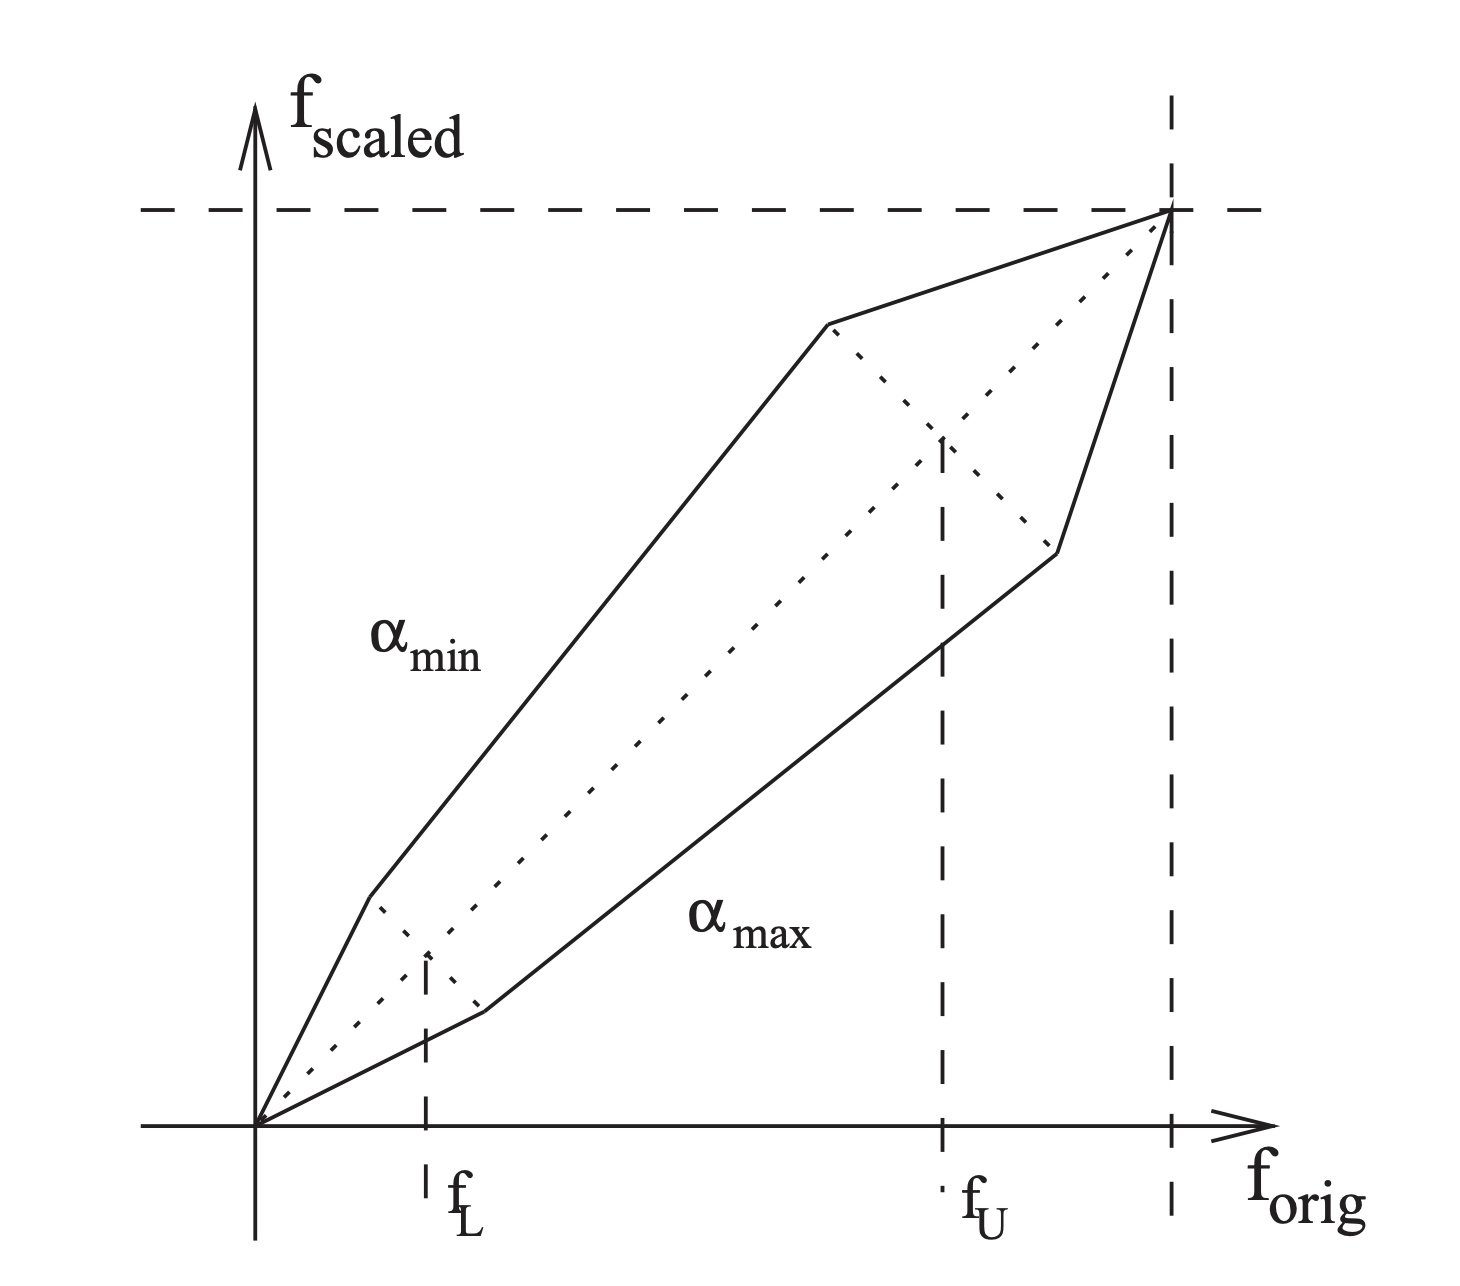
\includegraphics[width=0.52\textwidth]{imgs/wfunc_htk.png}}
\subfigure[VTLN frequency warping functions for a) linear, b) mel, and c) inverse mel frequency scales \cite{VTLN_wfun}]{\label{fig:notuse2}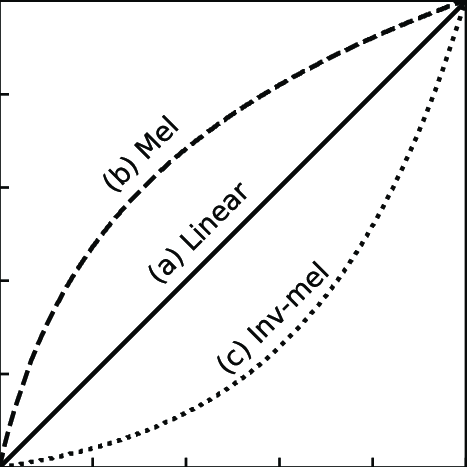
\includegraphics[width=0.4\textwidth]{imgs/wfun.png}}
\caption{Examples of  VTLN frequency warping functions}
\label{fig:wfun}
\end{figure}



% VTLN - Talk about limitation of VTLN
Another perspective to reduce children's acoustic variability is to work directly at the feature level, using standard feature extractors and directly adapting speech features to reduce children's acoustic variability. To this end, Vocal Track Length Normalization (VTLN) has been widely used to wrap spectral features into a canonical space \cite{VTLN, VTLN2}. Applied during the feature extraction process, after the windowing and Fourier transform, VTLN stretch or compress the frequency axis of the spectrum depending on a warping function (several examples of warping function are presented in figure \ref{fig:wfun}). As a result, the spectral representation of speaker variance is reduced, and children's speech features are normalised.
%f0 normlization and pitch normalized & Speaking rate adaptation
In addition, adapting acoustic models with Maximum Likelihood Linear Regression (MLLR) or Maximum A-Posteriori (MAP) and using Speaker adaptive training (SAT) based on feature MLLR (fMLLR) or Constrained MLLR (CMLLR) were found to be effective to improve the  performance of children ASR \cite{pronunciation, asr-improved2, children_language_model2, reviewASRchildren}.

Recently, some research explored normalising several aspects of speech: Pitch to reduce the spectral mismatch between children \cite{f0norm,pitchnorm,pitch_adapt_norm}, formant values to better match adult ones \cite{formant_norm} or speaking rate with a time-scale modification approach \cite{speaking_rate}.
Moreover, in accordance with the trend of shifting from knowledge to data drive framework, some recent studies attempted to use data-based feature adaptation. For example, \cite{adversarial-adapt1,adversarial-adapt2} used adversarial multi-task learning to produce age-invariant features which minimize the acoustic mismatch between adult and children's speech.

% MORE FEATURES
\subsubsection{Additional features}
In addition to feature extraction and feature-level adaptation, some research has demonstrated that concatenating speaker embeddings, such as i-vectors, to acoustic characteristics leads to more speaker-independent models \cite{ivector}.
Similarly, \cite{prosody_feat} proposes concatenating various prosodic variables such as loudness, voice intensity, and voice-probability to standard acoustic features, resulting in decreased inter-speaker variances and enhanced phoneme class discrimination.

\subsection{Detail of the annotation}
% age dependent subset
The material provided in speech corpora is frequently restricted to the audio signal, the corresponding text transcription, and some anonymised speaker's identifier. However, some additional information might be useful in improving children's speech recognition. The incorporation of the speaker's age would allow the development of age-dependent ASR systems in which the acoustical fluctuation caused by vocal track growth would be reduced \cite{linguistic-children}. 
% Level of transcription to tackle directly mispronunciation (subwords)
Some work showed the efficiency of an annotation at the sub-word level instead of the word level \cite{subwords} especially to be more robust to mistakes such as mispronunciations or hesitations.
% Phonetic dictionary with alternative pronunciation
Alternatively, in \cite{pronunciation,pronunciation2} user-dependent pronunciation lexicons are
employed to tackle the pronunciations divergence from the canonical and adult patterns.

% LM for children speech

\subsection{Structure of the acoustic model}%*******************************
The acoustic model is a key element in the recognition of children's speech since acoustic variability plays a major role in the degradation of children's speech recognition (compared to linguistic variability). As a result, the structure of the acoustic model is essential to be more robust to children's speech variability. In the rest of this section, we will review children's acoustic modelling structures in the context of hybrid models and end-to-end systems.
\subsubsection{Hybrid models}


\begin{figure}[ht]
\centering
\subfigure[]{\label{fig:TDNN}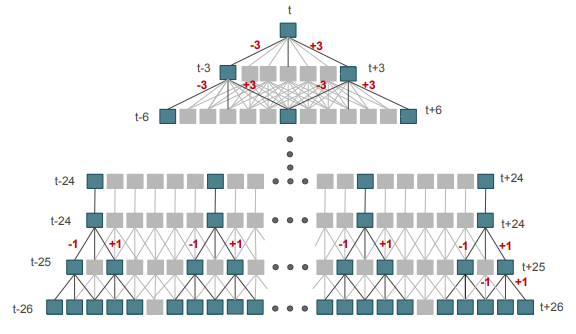
\includegraphics[width=0.48\textwidth]{imgs/TDNN.png}}
\subfigure[]{\label{fig:tdnnf}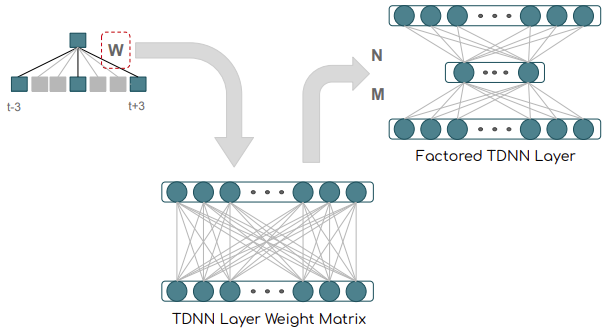
\includegraphics[width=0.48\textwidth]{imgs/TDNNF.png}}
\caption{(a) TDNN layers with sub-sampling \& (b) Factorized TDNN layer from \cite{TDNN-F}}
\end{figure}

%\begin{figure}
%    \centering
%    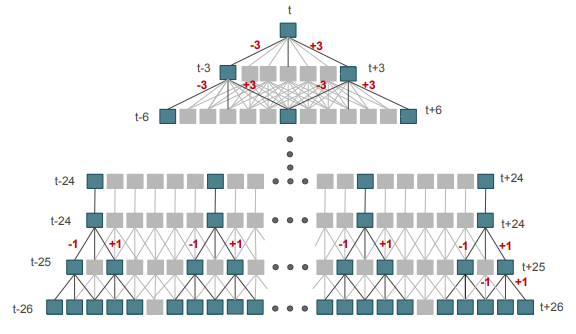
\includegraphics[width=1\textwidth]{imgs/TDNN.png}
%    \caption{TDNN with sub-sampling from \cite{TDNN-F}}
%    \label{fig:TDNN}
%\end{figure}
% Start with TDNN Cross entropy - standard (but more context, similar as CNN-1D)
Acoustic models for children generally follow the latest advances in acoustic modelling for adults. For example, \cite{TFchildren}  proposed switching from GMM to DNN for hybrid models. However, the traditional fully connected neural network does not provide the contextual information required for efficient phoneme recognition. Thus, time-delayed neural networks (TDNN) have been proposed (\cite{tdnn}). Working similarly to a one-dimensional convolutional neural network, where at each time step the current time step and its corresponding left and right context are provided, as shown in figure (\ref{fig:TDNN}). Additionally, the use of multiple layers of TDNN allows for the capture of broader contextual information, which leads to better phoneme recognition.
% TDNN-F
More recently, factorized time delay neural networks (TDNN-F) were introduced as a TDNN improvement \cite{TDNN-F} and proved to be effective for children ASR \cite{tdnnf-children}. They differ from TDNNs by applying a singular value decomposition (SVD) on the weight matrices $W$, which factorize them into two smaller rank matrices:
\begin{equation}
    W = U\Sigma V^T = MN
\end{equation}
Where $U$ is a  $m \times m$ complex unitary matrix, $\Sigma$ a  ${m\times n}$ non-negative rectangular diagonal matrix, $V$ a $n \times n$ complex unitary matrix, $M$ a $m \times k$ real matrix and $N$ a $k \times n$ real matrix.
With a suitable value of $k$ (much small than $m$ and $n$), this decomposition preserves the capabilities of the model, reduces the number of parameters and acts as a bottleneck layer (as shown in figure \ref{fig:tdnnf})

\subsubsection{End-to-end models}
% E2E and wav2vec
More recently, the ability of end-to-end models to outperform the hybrid HMM-DNN models in terms of absolute WER for children has been demonstrated \cite{gelin2021endtoend,sri_end2end,chen2020data,ng2020cuhk}. Nonetheless, a fundamental issue for this type of model is the requirement for a large amount of data to function correctly. Therefore, in most cases, training reliable end-to-end model for children from scratch is difficult. As a result, different training approaches are required, such as transfer learning (which will be detailed in further detail in section \ref{section:TL}) or semi and self-supervised learning, when there are few or no transcriptions, respectively \cite{xu21c_interspeech}.

\subsection{Data augmentation}%****************************************************
Deep learning's success is mostly due to its capacity to effectively utilise massive amounts of data to recognise patterns and be robust to variances. As a result, the lack of data on children's speech plays a significant part in performance deterioration as compared to adults. Data scarcity for children's speech is especially problematic for languages other than English, for which fewer resources are accessible in general. As a consequence, the need for large amounts of data has inspired research into a variety of data augmentation approaches, the goal of which is to artificially increase the amount of data for training.
There is two way of conducting this augmentation, according to the literature: using solely the data that is currently accessible or incorporating external data.

% With new data
\subsubsection{Using external data}
% Adult and children data -> Female speakers are more important
The use of out-of-domain adult data has been shown to be effective in improving the automatic recognition of children's speech \cite{adultAUGMENT1, adultAUGMENT2}. In particular, improvements were observed using adult female speech, as the acoustic mismatch between females and children is smaller than adult men.
%Children and children data
Similarly, \cite{nonnative} proposed to augment using directly additional children data.

%GAN and TTS
Furthermore, several studies proposed leveraging new data generated by deep learning systems as additional data during training. This is done in the literature using two families of algorithms: generative adversarial network (GAN) and text-to-speech (TTS). 


Generative Adversarial Networks are generative models that generate new data instances that are similar to the data on which they were trained. For that purpose, the GAN model is separated into two parts: a generator, which generates the synthetic data, and a discriminator, which receives either the created or actual data sample and attempts to differentiate between the two. During training, each module competes with the other, with the generator attempting to trick the discriminator and the discriminator attempting not to be fooled. A GAN was employed in \cite{GANS} to transform children's speech to adult speech in order to reduce variability. This was accomplished by feeding the generator children's utterances and utilising adult data as real data. In this approach, the discriminator seeks to differentiate between altered children's speech and real adult speech. At inference time, the discriminator is removed, leaving just the generator to turn children's speech into adult speech.


Text-to-speech systems aim to generate speech examples using directly the transcription as input. With recent advance of TTS systems such as Tacotron2 \cite{shen2018natural} or VITS \cite{kim2021conditional}, more realistic speech utterances are produced. Naturally, some research tried to use TTS outputs as data augmentation for ASR task \cite{laptev2020you} since the transcription and speech data are available. However, children's speech contains more complex traits than adults such as substandard or unclear pronunciation in addition to acoustics variability. As a result children's TTS quality is often inconsistent. In consequence, \cite{wang2021towards} proposed different data selection strategies such as speaker embedding similarity between the reference speaker and the speaker embedding extracted from generated speech utterance. With this data selection strategy, they have significantly reduced the CER for different children's speech recognition tasks.

% With actual data
\subsubsection{Using available data}
\begin{figure}
    \centering
    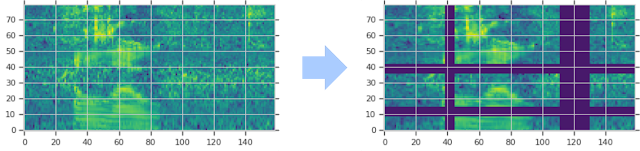
\includegraphics[width=1\textwidth]{imgs/specaugment.png}
    \caption{Before-After specaugment augmentation with warping of the time and time steps and Mel frequency masking (figure from \cite{specaugment})}
    \label{fig:specaugment}
\end{figure}
% Robustness with noise reverb
A common procedure for enhancing the robustness of the model by leveraging existing data is to construct a copy of the original data with different noises (such as babel noise, white noise, and music) and reverberation added \cite{liu2003noise,whitenoise,gelin2020babble,couvreur2000use,malek2017robust}. 
% Specaugment
More recently, vocal tract length perturbation (VTLP)\cite{VTLP} and spectral augmentation (SpecAugment) \cite{specaugment} became popular data augmentation techniques, in particular for end-to-end systems. They create a new copy of data by warping the frequency axis. SpecAugment also randomly masks time and frequency bands of the original audio at the feature level as shown in figure \ref{fig:specaugment}.

% Lucille work on mispronunciations
Finally, as mentioned in section \ref{subsection:mispron}, children's speech contains many disfluencies and errors which can complicate the learning process of the ASR model. Therefore, to make the model more robust to such errors, \cite{gelin2021simulating} proposed to synthetically create manual reading errors, such as word insertion or substitution by cutting the signal or adding speech elements produced by other children.





\subsection{Training procedure for children speech recognition}%******************************************

The most typical method for training a deep learning system is to alternate between forward and backward passes. The corpus input is supplied to the network in the forward pass to create a prediction. The loss is calculated using both predicted and actual target values. To reduce the number of prediction errors, network weights are adjusted using the gradient descent technique in the backpropagation phase. The model is considered trained after a number of loops between these two passes. There are, however, variations of this kind of pipeline in the literature such as transfer and multi-task learning, which stand out in the context of children's voice recognition.

% No example of semi-supervised for children, does not fit in this section
%Semi-supervised learning iteratively generates pseudo-labels with the current model, and uses those pseudo-labels to augment the training data and update the model \cite{semi}. Self-supervised learning. 



\subsubsection{Transfer learning}%************************************************************
\label{section:TL}

%Transfer learning (TL) or parameters transfer is a training procedure in which model parameters are initialized using knowledge gained from a model trained on a source related task. %(see figure \ref{fig:TL}).
%Transfer learning  (TL) or parameters transfer is a method, originally inspired by biological intelligence, which aims to use knowledge of source tasks as inductive bias during target task training. It can be seen as a system's ability to recognize and apply knowledge learned from previous tasks as a starting point for new tasks. In the context of machine learning, this transfer is applied at the parameters level. Model's parameters are initialized with parameters obtained from a model trained on a source related task, usually well-resourced.
When presented with a new problem in biological intelligence, people can employ information from a previous task as an inductive bias. Humans may avoid having to learn everything from scratch by transferring knowledge. It may be defined as the capacity to identify and utilise past task knowledge as a starting point for new tasks. In contrast, algorithms in machine learning are generally developed from scratch on a specific task. Transfer learning (TL) or parameters transfer is a concept that has emerged to bridge the gap between artificial and biological intelligence. To do this, the model's parameters are initialised with parameters obtained from another well-resourced model trained on a source-related task. Then, this model is adapted with the data from the new domain by adjusting the parameters to better fit the target task.
The resulting model leverages various underlying characteristics that have been captured by the different layers of the neural network during the training on the source domain step.
% during the learning process.
%More specifically, we consider a pre-trained acoustic model with a  set of parameters ${M_s}$ (including all layers, weight matrices, biases, activation functions, etc.) trained from source data $X_s$. Then, the output of this model is given by the forward pass $f(X_s;{M_s})$. $M_s$, is then adapted using the target data $X_t$ giving the adapted model $\widetilde{M_s}$. Thus, the output of the target forward pass would be $f(X_t; \widetilde{M_s})$.
A common assumption in deep learning is that the bottom layers, closest to the input, capture more signal-specific characteristics. While higher layers, near the output, capture task-specific information \cite{tfbased,yosinski2014transferable}. 
 % ++++ADVANTAGE OF TL +++++++
Furthermore, because the target model is based on a pre-trained model, one advantage of TL is that it requires less training data for adaptation.

\begin{figure}[t]
\centering
\subfigure[Acoustic adaptation]{\label{fig:acoustics_adapt}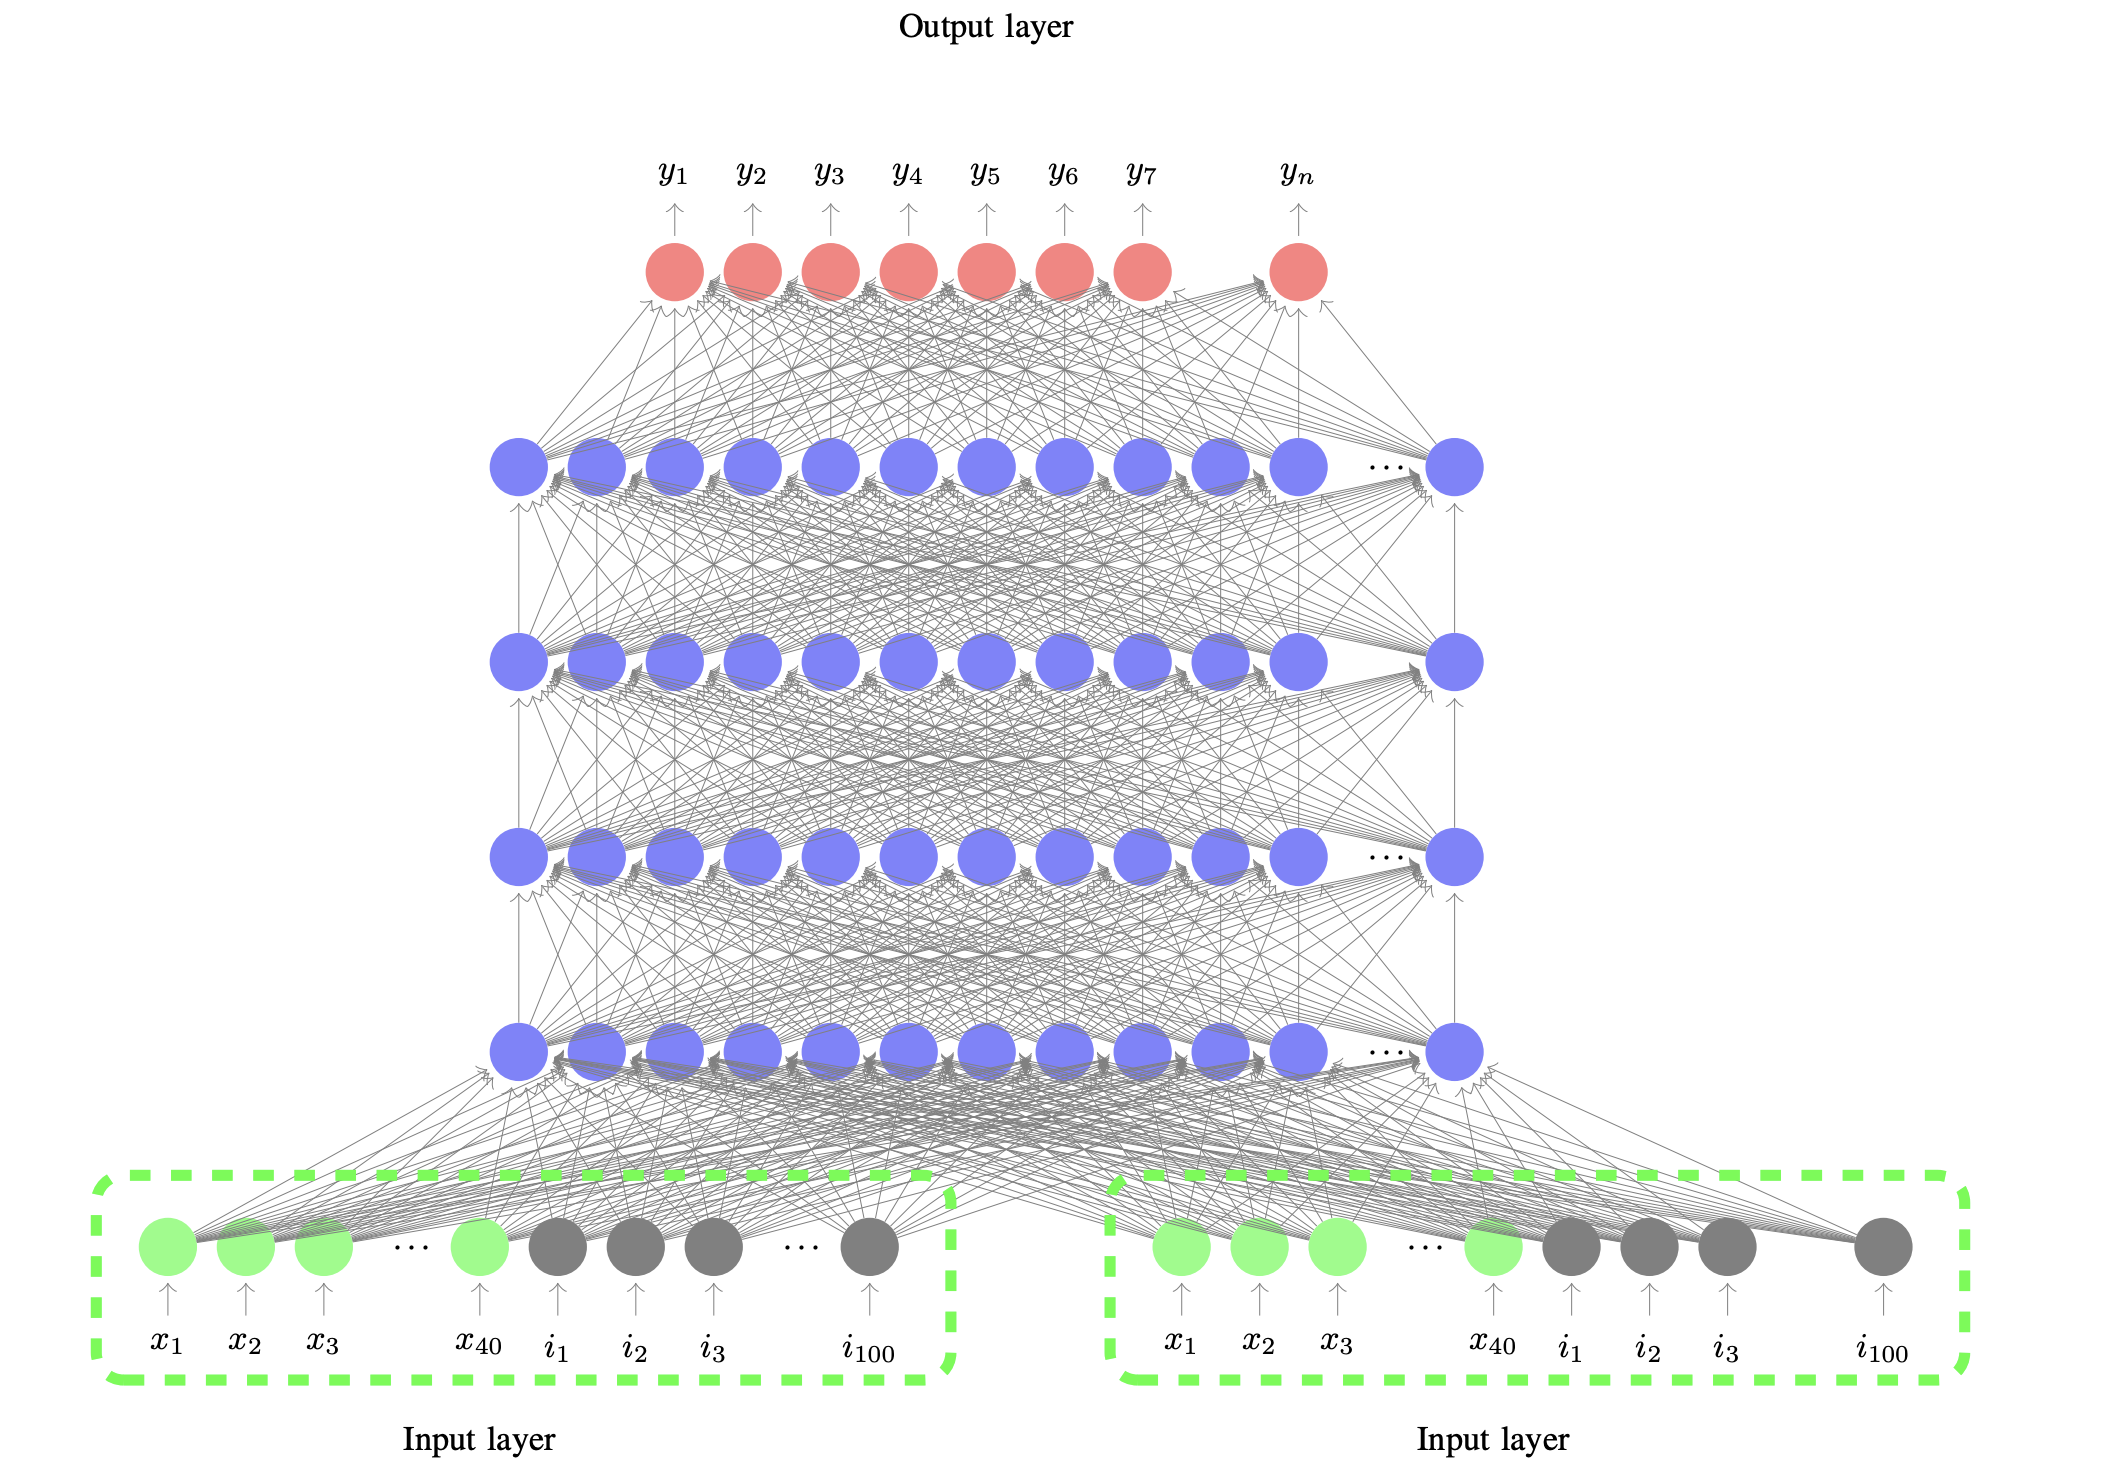
\includegraphics[width=0.48\textwidth]{imgs/tf_children.png}}
\subfigure[Pronunciation adaptation]{\label{fig:pronunciation_adapt}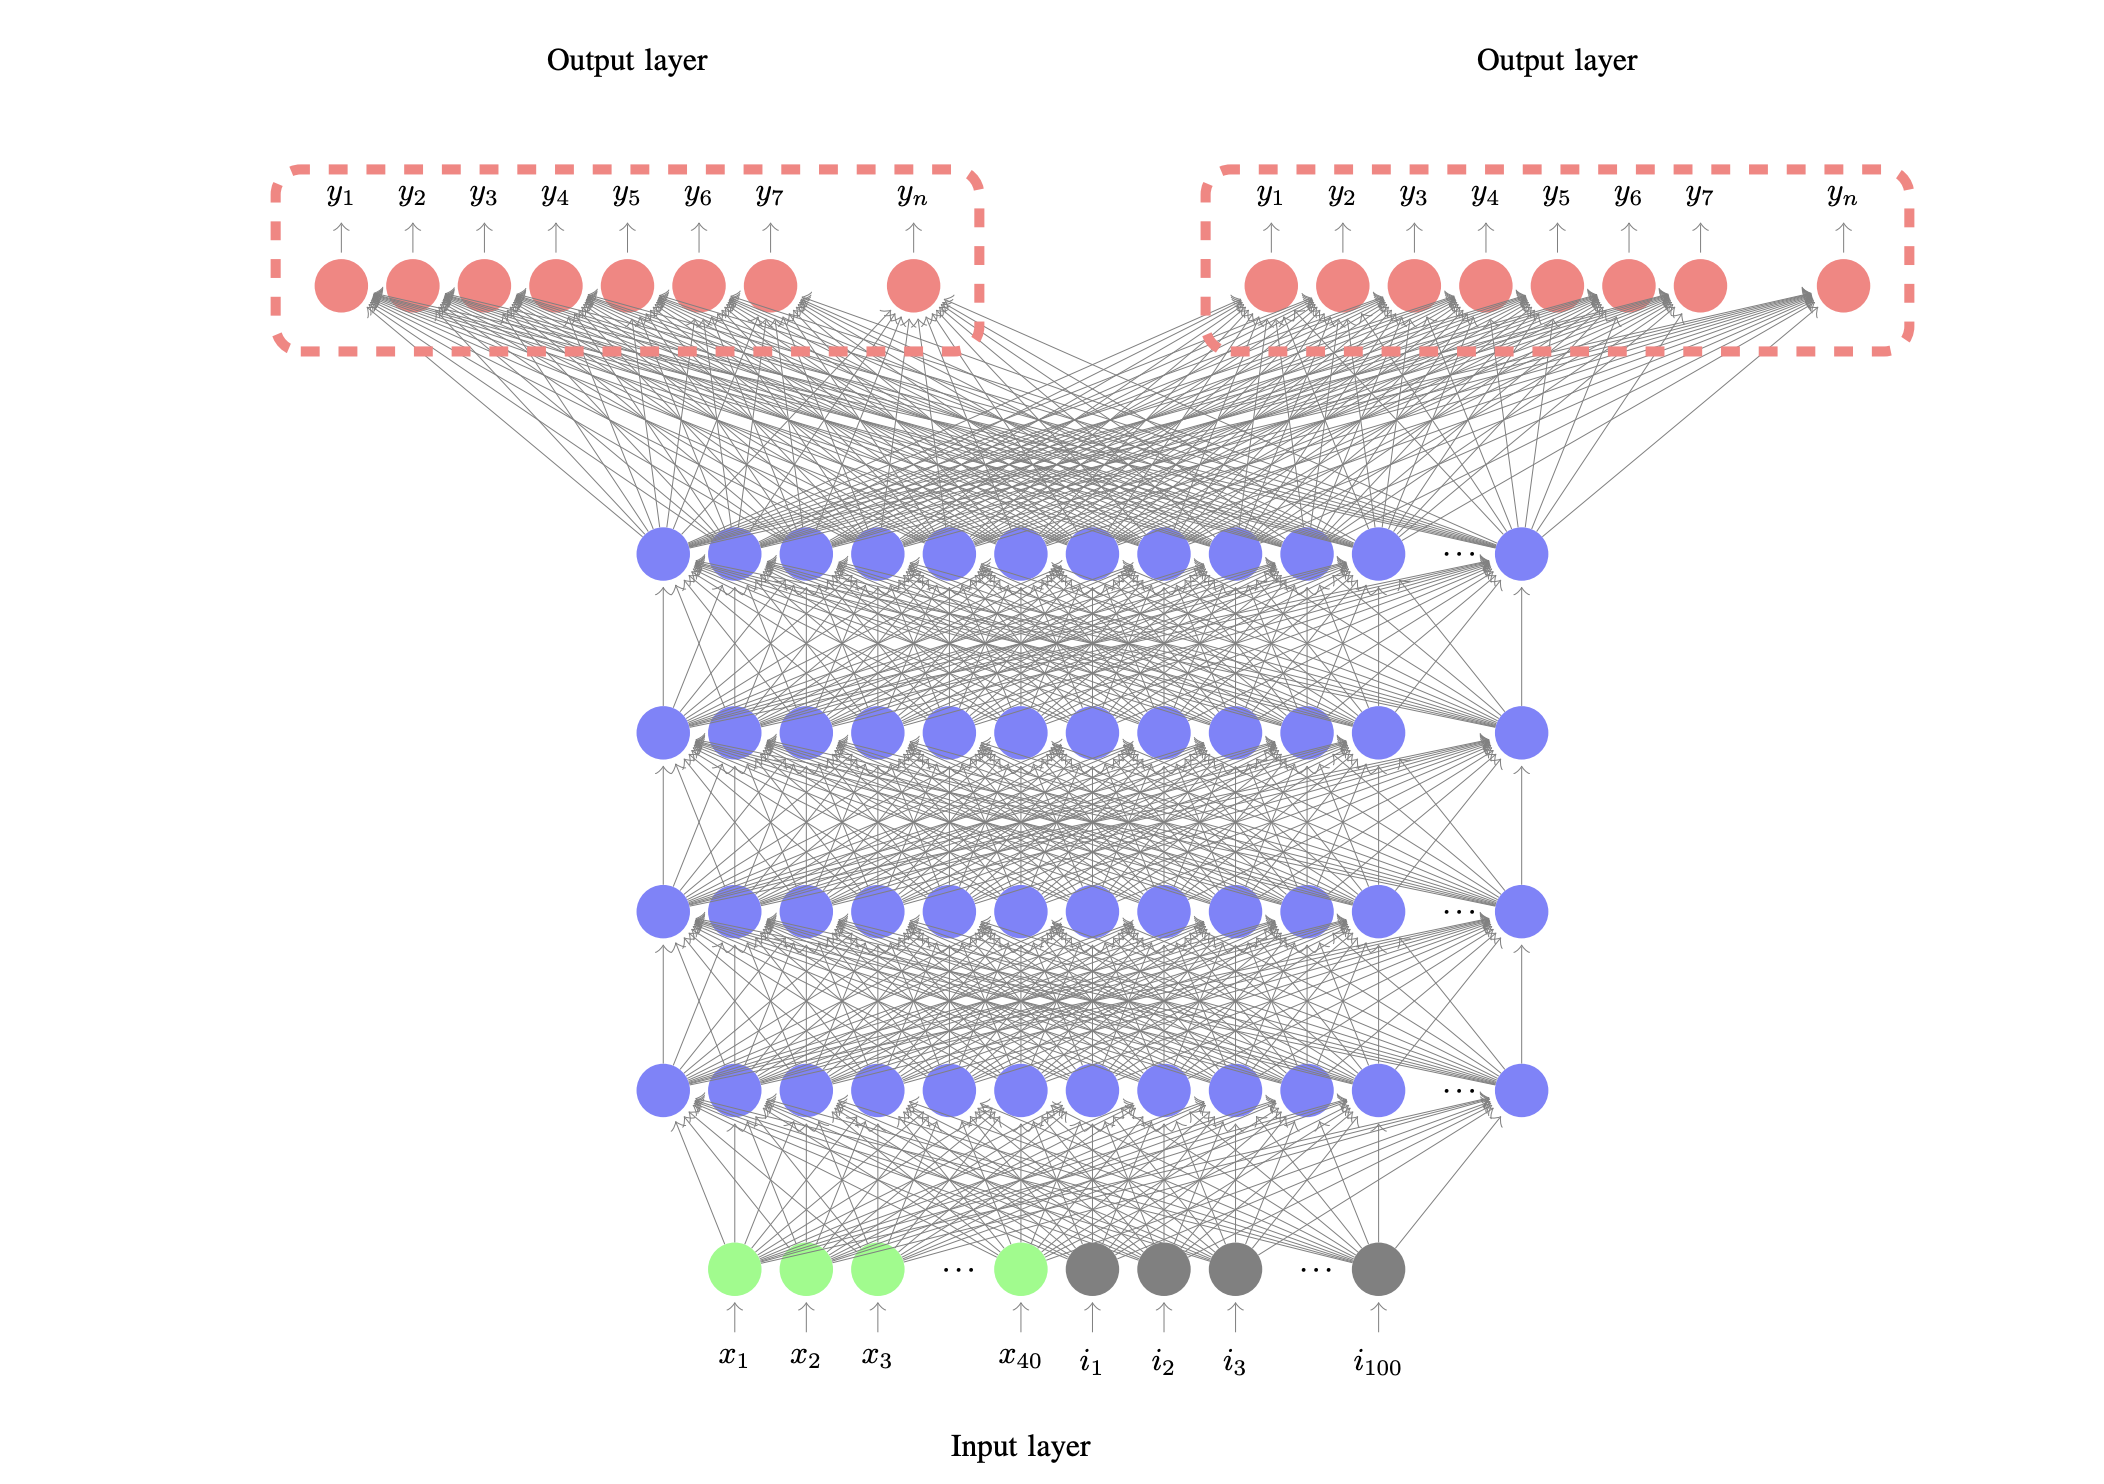
\includegraphics[width=0.48\textwidth]{imgs/pronunciation_adapt.png}}
\caption{Transfer learning approaches. Figures from \cite{TFchildren}}
\end{figure}

In recent years, TL has been successfully used in a wide variety of applications, especially for low-resource tasks, such as language understanding \cite{Bert}, character recognition \cite{tfcharacter} and dysarthric speech recognition \cite{tfpathology} among others. 
These successes have motivated its use for children's speech recognition. In particular, using large adults corpora as source domain. Indeed, recent acoustic models trained on adults are increasingly efficient and contain many acoustic and phonetic information that can be used for efficient adaptation to children's speech. Because children's speech variabilities are in both acoustics and pronunciation, \cite{TFchildren} proposed to study three different methods of TL to respectively access the contribution of acoustic adaptation, pronunciation adaptation and the combination of the two.

% Acoustic adaptation
Acoustic adaptation is based on the well-established idea that lower-level layers capture acoustic properties. In consequence, to solve children's acoustic variability that affects the lower-level layers, acoustic adaptation consists of freezing the top-level layer's weights and using TL on the lower-level layers as shown in figure \ref{fig:acoustics_adapt}. For \cite{TFchildren} and \cite{TransferLF}, acoustic transfer learning from an adult model for children, by retraining only the first layers of the model led to respectively 38\% and 26\% WER relative improvements compared to adult models performances. Furthermore, with a 4.9\% relative WER improvement, the children's acoustic adaption outperforms a randomly initialised acoustic model trained on the same children's data.

% Pronunciation adaptation
Pronunciation adaptation is based on the assumption that higher-level layers capture task characteristic information, which in the context of ASR is pronunciation. Pronunciation is the act or manner of pronouncing words using phonetic symbols, phonetic symbols which correspond to the different outputs of the acoustic model. Pronunciation adaptation, as illustrated in figure \ref{fig:pronunciation_adapt}, adapt higher layer, keeping lower-level layers weight frozen. In \cite{TFchildren}, pronunciation adaptation on the last layers of the model led to 31\% relative WER improvement compared to the adult model's performance. However, as compared to a randomly initialised acoustic model trained with the same children's data, pronunciation adaptation degrades by 5.6\% relative WER.

% Combination of acoustic and pronunciation / TL on all layers
Finally, fine-tuning the entire network outperforms both acoustic and pronunciation adaptation alone. Similar findings have recently been seen in end-to-end models, where TL leveraging an adult pre-trained model outperformed training from scratch using only children's data \cite{sri_end2end,gelin2021endtoend}. 
% Multi-task
\subsubsection{Multi-task learning}%************************************************************
\label{section:MTL}
\begin{figure}[t]
\begin{center}

\includegraphics[width=0.7\textwidth]{imgs/MTL.png}
\caption{Multilingual approach using each language as a task in a multi-task learning context.}
\label{fig:MTL}
\end{center}
\end{figure}

Multi-task learning (MTL), like transfer learning, is inspired by biological intelligence. By training all tasks in simultaneously, MTL tries to discover shared representations between related tasks. MTL differs from TL in that it does not limit learning to only the source and target tasks in sequential training, but instead permits learning with as many tasks as possible in parallel.  In general, a typical MTL model consists of two different parts. The first part is the sub-network shared by all tasks, while the second is a task-specific output sub-network (see figure \ref{fig:MTL}). The joint representation learned in the shared layers is more robust, allowing the model to be more reliable.  
More formally, for any task $i$ the corresponding output of the forward pass will be:
\begin{equation} \label{equation:MT}
    f(X_i;\{M_i, M_{c}\}) = f_i(f_{c}(X_i,{M_{c}}); {M_i}) 
\end{equation}
where $X_i$ is the data associated with the task $i$, $M_i$ represents the task-specific parameters of the model, and $M_{c}$ corresponds to the parameters that are shared (or common) across all tasks.

Therefore, the performances of the MTL greatly depends on the task-relatedness. Indeed, the MTL is sensitive to outlier tasks that are unrelated to the rest of the tasks. This is due to the difficulty to learn common representations for tasks that are unrelated to each other \cite{zhang2018overview}.

MTL has been used effectively in a variety of areas, including natural language processing \cite{multi-nlp}, computer vision \cite{mtl_computervision} and bioinformatics \cite{bioinfo}. MTL has been naturally applied in the field of automatic speech recognition \cite{MTL-LFMMI} with directly application to low-resource ASR \cite{abad2020}. Given that child ASR is a resource-limited task, MTL has been proposed to address the issue of data scarcity by utilising various datasets of children's speech. 
 \cite{TransferLF} and \cite{2019multi} successfully applied MTL to Mandarin and English-speaking children, with a 16.96\% relative improvement in WER for the English children.


\section{Children Corpora}
\label{section:children_corpora}
As described in chapter \ref{section:data_scarcity}, notwithstanding recent efforts to collect databases on children's speech, there are still fewer data available than for adults. In addition, collecting speech data for children is challenging in many ways, from the child's attention span, mispronunciations, and ungrammatical expression to the use of out-of-ordinary words. Therefore, the scarcity of publicly available child speech corpora and their small size impeded research and further development of reliable ASR systems for children. 


\begin{table}
%\centering
\small
\begin{tabular}{l|c|c|c|c|c|c} 
\hline
\multicolumn{1}{c|}{\textbf{Corpus}} & \multicolumn{1}{c|}{\textbf{Languages}} & \multicolumn{1}{c|}{\textbf{\# Spkrs}} & \multicolumn{1}{c|}{\textbf{\# Utt}} & \multicolumn{1}{c|}{\textbf{Dur.}} & \multicolumn{1}{c|}{\textbf{Age Range}} & \multicolumn{1}{c}{\textbf{Date}} \\ 
\hline
Providence Corpus \cite{providence} & English & 6 &  & 363h & 1-3 & 2006 \\ 
\hline
Lyon Corpus \cite{LyonSC} & French & 4 &  & 185h & 1-3 & 2007 \\ 
\hline
CASS\_CHILD \cite{cass_child} & Mandarin & 23 &  & 631h & 1-4 & 2012 \\ 
\hline
Demuth Sesotho Corpus \cite{demuth1992acquisition} & Sesotho & 4 & 13250 & 98h & 2-4 & 1992 \\ 
\hline
NITK Kids’ Speech Corpus \cite{nitk} & Kannada & 160 &  & 10h & 2-6 & 2019 \\ 
\hline
CHIEDE \cite{chiede} & Spanish & 59 & 15,444 & 8h & 3-6 & 2008 \\ 
\hline
CUChild \cite{cuchild} & Cantonese & 1,986 &  &  & 3-6 & 2020 \\ 
\hline
EmoChildRu \cite{emochildru} & Russian & 100 & 20,000 & 30h & 3-7 & 2015 \\ 
\hline
CNG Portuguese children\cite{hamalainen2013cng} & Portuguese & 510 &  & 21h & 3-10 & 2013 \\ 
\hline
AusKidTalk$^1$ \cite{ahmed2021auskidtalk} & English & 750 &  & 600h & 3-12 & 2021 \\ 
\hline
\textbf{PF-STAR-SWEDISH} \cite{pfstar}
& Swedish & 198 & 8,909 & 6h & 4-8 & 2005 \\ 
\hline
PF-STAR Children British \cite{pfstar,russell2006pf,pf-star-british} & English & 158 &  & 14.5h & 4-14 & 2006 \\ 
\hline
AD-child. RU \cite{ad-child_ru} & Russian & 278 &  &  & 4-16 & 2019 \\ 
\hline
TBALL \cite{tball} & English & 256 & 5,000 & 40h & 5-8 & 2005 \\ 
\hline
SPECO \cite{speco} & Hungarian & 72 &  & 12h & 5-11 & 1999 \\ 
\hline
UltraSuite\cite{eshky2019ultrasuite} & English & 86 & 14,456 & 37h & 5-14 & 2019 \\ 
\hline
CID read speech corpus \cite{lee1999acoustics} & English & 436 &  &  & 5-18 & 1996 \\ 
\hline
Persian Kids Speech Corpus \cite{khanzadi2022persian} & Persian & 286 & 162,395 & 33h & 6-9 & 2022 \\ 
\hline
\textbf{Letsread$^2$} \cite{letsread} & Portuguese & 284 & 4,629 & 14h & 6-10 & 2016 \\ 
\hline
\textbf{CMU kids Corpus} \cite{cmu} & English & 76 & 5,180 &  & 6-11 & 1997 \\ 
\hline
CFSC \cite{CFSC} & Filipino & 57 &  & 8h & 6-11 & 2012 \\ 
\hline
IESC-Child \cite{PEREZESPINOSA202055} & Spanish & 174 & 19,793 & 34h & 6-11 & 2020 \\ 
\hline

CU Children's read and prompted \cite{hagen2003children}& English & 663 & 66300 &  & K-G5 & 2001 \\ 
\hline
\textbf{Chorec$^2$} \cite{chorec} & Dutch & 400 & 3,065 & 25h & 6-12 & 2008 \\ 
\hline
ChildIt2 \cite{childit2} & Italian & 96 &  4,875 & 9h & 6-14 & 2016 \\ 
\hline
TIDIGITS \cite{leonard1993tidigits} & English & 101 &  &  & 6-15 & 1993 \\ 
\hline
CSLU Kids' Speech Corpus \cite{cslu} & English & 1,100 & 1,017 &  & K-G10 & 2007 \\ 
\hline
SingaKids-Mandarin \cite{singakids} & Mandarin & 255 & 79,843 & 125h & 7-12 & 2016 \\ 
\hline
ChildIt corpus \cite{gerosa2006acoustic} & Italian & 171 &  &  & 7-13 & 2007 \\ 
\hline
VoiceClass Database \cite{burkhardt2010database} & German & 170 &  &  & 7-14 & 2010 \\ 
\hline
Deutsche Telekom telephone \cite{burkhardt2010database} & German & 106 &  &  & 7-14 & 2010 \\ 
\hline
Jasmin \cite{JASMIN} & Dutch &  &  & 63h & 7-16 & 2008 \\ 
\hline
Tgr-child corpus \cite{gerosa2006acoustic} & Italian & 30 &  &  & 8-12 & 2007 \\ 
\hline
SponIt corpus \cite{gerosa2006acoustic} & Italian & 21 &  &  & 8-12 & 2007 \\ 
\hline
Swedish NICE Corpus \cite{bell2005swedish} & Swedish & 75 & 5,580 &  & 8-15 & 2005 \\
\hline
CHIMP spontaneous speech \cite{language_children2} & English & 160 &  &  & 8-14 & 2002 \\ 
\hline
SpeeCon corpus  \cite{SPEECONS} & 20 Languages &  &  &  & 8-15 & 2002 \\ 
\hline
Rafael.0 telephone corpus \cite{linguistic-children} & Danish & 306 &  &  & 8-18 & 1996 \\ 
\hline
\textbf{Boulder Learning - MyST} \cite{MyST} & English & 1,371 & 228,874 & 384h & G3-G5 & 2019 \\ 
\hline
CU Story Corpus \cite{hagen2003children} & English & 106 & 5,000 & 40h & G3-G5 & 2003 \\ 
\hline
\textbf{ETLT$^2$} \cite{etlt} & L2 German &  & 1,674 & 6h & 9-16 & 2020 \\ 
\hline
Lesetest corpus \cite{grissemann2000zurcher} & German & 62 &  &  & 10-12 & 2000 \\ 
\hline
FAU Aibo Emotion Corpus \cite{steidl2009automatic} & German & 51 & 13,642 & 9h & 10-13 & 2002 \\ 
\hline
PIXIE corpus \cite{bell2003child} & Swedish & 2,885 &  &  &  & 2003 \\ 
\hline
Takemaru-kun corpus \cite{takemaru} & Japanese & 17,392 &  &  & & 2007 \\ 
\hline
CALL-SLT \cite{callslt} & German &  & 5,000 &  &  & 2014 \\ 
\hline
\multicolumn{7}{l}{$^1$ At the day of this proposal, data collection for this dataset is not complete.} \\
\multicolumn{7}{l}{$^2$ Information displayed here correspond to a subset of the original data used in this proposal.}  \\
\end{tabular}
\caption{Non-exhaustive comparison of children's speech corpora. This table has been sorted by age range. Blanks indicate unavailable information. Entries highlighted in bold correspond to the corpora used in the experiments presented in this PhD thesis proposal. K: Kindergarden. G: Grade}
\label{table:children_corpora}
\end{table}
Table \ref{table:children_corpora} provides a list of existing corpora of children's speech. Notably, one-third of the available corpora are in English. Similarly, one-third is focused to children under the age of 4. Furthermore, there is always a trade-off between speaker diversity, total duration, and utterance number.

The remainder of this section will go through the children's speech corpora that were used in this proposal.

\subsection{LETSREAD}
LetsRead database \cite{letsread} is a read-aloud speech database of European Portuguese from children aged 6 to 10,  from 1st to 4th grade. This corpus is composed of a total of 284 children, 147 girls and 137 boys, whose mother tongue is European Portuguese. Children from private and public Portuguese schools were asked to carry out two tasks: reading sentences and a list of pseudo-words. The difficulty of the tasks varies depending on the school year of the child. 
For this proposal, we excluded all utterances from the pseudo-word reading task because we do not include pseudo-words in the language model and lexicon in our experiments. 
\subsection{PFSTAR\_SWEDISH}
The PFStar children's speech corpus \cite{pfstar} was collected as part of the EU FP5 PFSTAR project. It contains more than 60 hours of speech. This corpus is divided into two parts: native-language speech and non-native language part.
The native-language speech part contains recordings of British English, German and Swedish children, from 4 to 14 years old. The non-native language part consists of speech by Italian, German and Swedish children speaking English. In this work, we only used the native language Swedish part, consisting of speech by 198 native Swedish children, between 4 and 8 years old recorded in the Stockholm area, imitating an adult who read the text from a screen.
\subsection{ETLTDE}
Extended Trentino Language Testing (ETLT) corpus \cite{etlt} has been collected in northern Italy for assessing English and German proficiency of Italian children between 9 and 16 years old, by asking them to answer questions. The data collection was carried out in schools. On average the signal quality is good, but some background noise is often present (doors, steps, keyboard typing, background voices, street noises if the windows are open, etc). In addition, many answers are whispered and difficult to understand.
For this proposal, we only used the German-transcribed subset (named ETLTDE), around 6h divided into training and test partitions.
\subsection{CMU\_KIDS}
The CMU kids corpus \cite{cmu} contains English sentences read aloud by children, 24 males and 52 females, from 6 to 11 years old. In total, 5,180 utterances were recorded with one sentence per utterance. This database was created to train the SPHINX II \cite{sphinx2} automatic speech recognition system within the LISTEN project at Carnegie Mellon University (CMU).
\subsection{CHOREC}
\label{subsection:chorec}
The Chorec corpus \cite{chorec} consists of 400 Dutch-speaking elementary school children, between 6 and 12 years old, reading words, pseudo-words and stories. The difficulty of the reading task was adapted to children with 9 different levels. Recordings were made in schools, leading to some environmental noises (school bells, children entering the playground etc.). For this proposal, similarly to the LETSREAD dataset, we discarded pseudo-word utterances.

\subsection{MyST}
My Science Tutor (MyST) Children Speech Corpus \cite{MyST} is currently one of the largest publicly available corpora of English children's speech, with around 400 hours. This is about 10 times more than all other English children's speech corpora combined. It consists of conversations between children and a virtual tutor in 8 scientific domains. Speech was collected from 1,372  students in third, fourth and fifth grades. Partitioning of the corpus is already available, ensuring reasonably representation of each scientific domain and that each student is present in only one partition. However, only 45\% of the utterances were transcribed at the word level. Furthermore, for the purposes of this proposal, we decided to remove all utterances shorter than one second and longer than 30 seconds. After this filtering, 81971 utterances from 736 speakers for a total of 151 hours remain.


\section{Summary}
In this chapter, we provided a brief overview of children's automatic speech recognition, its challenges, and the research community's response. Indeed, ASR in children has long been acknowledged as challenging. This is mostly due to the development of the vocal apparatus, which produces an acoustic gap with adult speech; nonetheless, this mismatch diminishes until the age of 15. Despite all efforts, it remains an active and challenging area of research. In this chapter, we also discussed inductive bias approaches, such as transfer learning and multi-task learning, which would be applied in the work detailed in this proposal. Furthermore, we present the most complete comparison of children's speech corpora to our knowledge.